\documentclass[11pt]{SANDreport}

%Local stuff
%\usepackage{latexsym}
%
% Put a DRAFT watermark in your document that works with pdflatex!
%

% Taken from http://jeanmartina.blogspot.com/2008/07/latex-goodie-how-to-watermark-things-in.html

\usepackage{graphicx,type1cm,eso-pic,color}

\makeatletter
\AddToShipoutPicture{%
\setlength{\@tempdimb}{.5\paperwidth}%
\setlength{\@tempdimc}{.5\paperheight}%
\setlength{\unitlength}{1pt}%
\put(\strip@pt\@tempdimb,\strip@pt\@tempdimc){%
\makebox(0,0){\rotatebox{45}{\textcolor[gray]{0.95}%
{\fontsize{6cm}{6cm}\selectfont{DRAFT}}}}%
\makebox(-100,-300){\rotatebox{45}{\textcolor[gray]{0.95}%
{\fontsize{2cm}{2cm}\selectfont{Internal Use}}}}
%\makebox(-500,-0){\rotatebox{90}{\textcolor[gray]{0.95}%
%{\fontsize{0.7cm}{0.7cm}\selectfont{\textcopyright Copyright 2008 - Jean Martina}}}}
}%
}
\makeatother


\usepackage[colorlinks]{hyperref}
\usepackage{color}
\usepackage{graphicx}
\usepackage{wrapfig}


\usepackage{listings}
\usepackage[compact]{titlesec}
\usepackage{mdwlist}

\usepackage{paralist}

%\usepackage{makeidx}
%\makeindex

%
% Command to print 1/2 in math mode real nice
%
\newcommand{\myonehalf}{{}^1 \!\!  /  \! {}_2}

%
% Command to print over/under left aligned in math mode
%
\newcommand{\myoverunderleft}[2]{ \begin{array}{l} #1 \\ \scriptstyle #2 \end{array} }

%
% Command to number equations 1.a, 1.b etc.
%
\newcounter{saveeqn}
\newcommand{\alpheqn}{\setcounter{saveeqn}{\value{equation}}
\stepcounter{saveeqn}\setcounter{equation}{0}
\renewcommand{\theequation}
	{\mbox{\arabic{saveeqn}.\alph{equation}}}}
\newcommand{\reseteqn}{\setcounter{equation}{\value{saveeqn}}
\renewcommand{\theequation}{\arabic{equation}}}

%
% Shorthand macros for setting up a matrix or vector
%
\newcommand{\bmat}[1]{\left[ \begin{array}{#1}}
\newcommand{\emat}{\end{array} \right]}

%
% Command for a good looking \Re in math enviornment
%
\newcommand{\RE}{\mbox{\textbf{I}}\hspace{-0.6ex}\mbox{\textbf{R}}}

%
% Commands for Jacobians
%
\newcommand{\Jac}[2]{\displaystyle{\frac{\partial #1}{\partial #2}}}
\newcommand{\jac}[2]{\partial #1 / \partial #2}

%
% Commands for Hessians
%
\newcommand{\Hess}[2]{\displaystyle{\frac{\partial^2 #1}{\partial #2^2}}}
\newcommand{\hess}[2]{\partial^2 #1 / \partial #2^2}
\newcommand{\HessTwo}[3]{\displaystyle{\frac{\partial^2 #1}{\partial #2 \partial #3}}}
\newcommand{\hessTwo}[3]{\partial^2 #1 / (\partial #2 \partial #3)}



%\newcommand{\Hess2}[3]{\displaystyle{\frac{\partial^2 #1}{\partial #2 \partial #3}}}
%\newcommand{\myHess2}{\frac{a}{b}}
%\newcommand{\hess2}[3]{\partial^2 #1 / (\partial #2 \partial #3)}

%
% Shorthand macros for setting up a single tab indent
%
\newcommand{\bifthen}{\begin{tabbing} xxxx\=xxxx\=xxxx\=xxxx\=xxxx\=xxxx\= \kill}
\newcommand{\eifthen}{\end{tabbing}}

%
% Shorthand for inserting four spaces
%
\newcommand{\tb}{\hspace{4ex}}

%
% Commands for beginning and ending single spacing
%
\newcommand{\bsinglespace}{\renewcommand{\baselinestretch}{1.2}\small\normalsize}
\newcommand{\esinglespace}{}


\setcounter{tocdepth}{3}

\raggedright

% If you want to relax some of the SAND98-0730 requirements, use the "relax"
% option. It adds spaces and boldface in the table of contents, and does not
% force the page layout sizes.
% e.g. \documentclass[relax,12pt]{SANDreport}
%
% You can also use the "strict" option, which applies even more of the
% SAND98-0730 guidelines. It gets rid of section numbers which are often
% useful; e.g. \documentclass[strict]{SANDreport}

% ---------------------------------------------------------------------------- %
%
% Set the title, author, and date
%

\title{\center
Trilinos Lifecycle Model \\[2ex] Version 2.0 \\[2ex] \large A
Lean/Agile Software Lifecycle Model for Research-based Computational
Science and Engineering and Applied Mathematical Software }
\author{
Roscoe A. Bartlett \\ Oak Ridge National Laboratories\footnote{Oak
Ridge National Laboratories is Managed by UT-Battelle, a partnership
of the University of Tennessee and Battelle Memorial Institute, for
United States Department of Energy under Contract DE-AC05-00OR22725.} 
\\[2ex] Mike Heroux \\ Jim Willenbring \\ Sandia
National Laboratories\footnote{Sandia is a multiprogram laboratory
operated by Sandia Corporation, a Lockheed-Martin Company, for the
United States Department of Energy under Contract DE-AC04-94AL85000.},
Albuquerque NM 87185 USA, \\ }
\date{}

% ---------------------------------------------------------------------------- %
% Set some things we need for SAND reports. These are mandatory
%
\SANDnum{SAND2012-XXXX}
\SANDprintDate{January ???}
\SANDauthor{
Roscoe A. Bartlett \\ Mike Heroux \\ Jim Willenbring }

% ---------------------------------------------------------------------------- %
% The following definitions are optional. The values shown are the default
% ones provided by SANDreport.cls
%
\SANDreleaseType{Unlimited Release}
%\SANDreleaseType{Not approved for general release}

% ---------------------------------------------------------------------------- %
% The following definition does not have a default value and will not
% print anything, if not defined
%
%\SANDsupersed{SAND1901-0001}{January 1901}

%
% Glossary
%

%\makeglossaries
%\newglossaryentry{value_type}{name={Value Type},
%description={A concrete built-in or user-defined (class) type that has a
%public default constructor, copy constructor, and assignment operator.  Value
%type objects typically have a small memory footprint which allows them to be
%copied without excessive overhead.}


% ------------------------------------------------------------------------- %
%
% Start the document
%
\begin{document}

\pagenumbering{roman}

\maketitle

% ------------------------------------------------------------------------ %
% An Abstract is required for SAND reports
%

%
\begin{abstract}
%

Software lifecycle is becoming an increasing important issue for
computational science \& engineering (CSE) and applied mathematical
software.  The process by which a piece of CSE software begins life as
a product of a research effort and then matures into a trusted
high-quality capability is a vexing problem for the CSE community.
Here we describe a proposal for a well-defined software lifecycle
process based on modern Lean/Agile software engineering principles
that is appropriate for many CSE software projects that are initially
heavily focused on research but also are expected to eventually
produce usable high-quality capabilities.  Here, three different
phases/maturity levels are advocated for the transition from research
to production software that consider the appropriate handling of many
issues.  The goals of this lifecycle model are to better communicate
maturity levels with customers and to help to identify and promote SE
practicies that will help to improve productivity and produce better
software.  An important collection of software in this domain is
Trilinos which is used as the motivation and the initial target for
this lifecycle model.  However, many other related and similar CSE
(and non-CSE) software projects might also make good use of this
lifecycle model.  Indeed this lifecycle process, if followed, would
allow for very large-scale sustainable integration of large amounts of
complex CSE software efforts across many different institutions.

%
\end{abstract}
%

% ------------------------------------------------------------------------ %
% An Acknowledgement section is optional but important, if someone made
% contributions or helped beyond the normal part of a work assignment.
% Use \section* since we don't want it in the table of context
%
%\clearpage
%\section*{Acknowledgment}
%
%
%The format of this report is based on information found
%in~\cite{Sand98-0730}.

% ------------------------------------------------------------------------ %
% The table of contents and list of figures and tables
% Comment out \listoffigures and \listoftables if there are no
% figures or tables. Make sure this starts on an odd numbered page
%
\clearpage
\tableofcontents
%\nopagebreak\listoffigures
%\nopagebreak\listoftables

% ---------------------------------------------------------------------- %
% An optional preface or Foreword
%\clearpage
%\section{Preface}
%Although muggles usually have only limited experience with
%magic, and many even dispute its existence, it is worthwhile
%to be open minded and explore the possibilities.

% ---------------------------------------------------------------------- %
% An optional executive summary
%\clearpage
%\section{Summary}
%Once a certain level of mistrust and scepticism has
%been overcome, magic finds many uses in todays science
%and engineering. In this report we explain some of the
%fundamental spells and instruments of magic and wizardry. We
%then conclude with a few examples on how they can be used
%in daily activities at national Laboratories.

% ---------------------------------------------------------------------- %
% An optional glossary. We don't want it to be numbered
%\clearpage
%\section*{Nomenclature}
%\addcontentsline{toc}{section}{Nomenclature}
%\begin{itemize}
%\item[alohomora]
%spell to open locked doors and containers
%\end{itemize}

% ---------------------------------------------------------------------- %
% This is where the body of the report begins; usually with an Introduction
%
\SANDmain % Start the main part of the report

\pagenumbering{arabic}

%
\section{Introduction and Background}
%

{}\textbf{ToDos:}

\begin{compactenum}

  {}\item (Ross B.) Call this the ``TriBITS Lifecycle Model'' and just
  Trilinos in the abstract and the text.
1
  {}\item (Jim W.) Improve structure of the risk analysis section.  This
  should start with a set of bullets for the various risks being mentioned,
  followed by a sort discussion of why self-sustaining software helps to
  address many of these risks automatically, and then followed by more
  detailed discussion of each risk along with mitigation ideas.

  {}\item (Mike H.) Go over the entire document and made edits and
  restructures, etc.

  {}\item (Ross B., Jim W., and Mike H.) Read over document, make notes, and
  discuss the final revisions to be made.

  {}\item Send out final draft to Trilinos developers for review.

  {}\item Get back comments and incorprate feedback as apprpriate.

  {}\item Discuss final draft, decide on and make any final revisions, and
  then publish the SAND report.

\end{compactenum}

\begin{wrapfigure}{r}{0.5\textwidth}
\begin{center}
\fbox{
\begin{minipage}[b]{0.45\textwidth}
\raggedright
The {}\textit{Trilinos Project} is an effort to facilitate the design,
development, integration and on-going support of foundational
libraries for computational science and engineering applications.
Trilinos is composed of a set of different packages with a wide range
of capabilities including basic distributed memory linear algebra,
load balancing, discretization support, and wide variety of nonlinear
analysis methods and much more.  Trilinos packages have complex
dependencies on each other and create a challenging software
development environment.  The primary programming language for
Trilinos is C++ and therefore C++ considerations dominate Trilinos
development.
\end{minipage}
} %fbox
\end{center}
\end{wrapfigure}

Computational Science and Engineering (CSE) is experiencing a
challenge in software lifecycle issues.  Much software in CSE begins
development as research software but at some point begins to be used
in other software and is desired (or is expected) to eventually
achieve production-quality.  There is currently no sufficient software
engineering lifecycle model defined for these types of CSE software
that has been shown to be effective.  A previous attempt to create a
viable lifecycle model for Trilinos to provide for transitions of CSE
software from research, to production, to maintenance (and later
death) was defined in {}\cite{TrilinosLifecycleModel2007}.  Since then we
have continued learning more effective techniques for software engineering.
This present lifecycle model reflects what we have learned.

The goals for defining a lifecycle model for Trilinos are many but the
most important include:

\begin{compactitem}

{}\item\textit{Allow Exploratory Research to Remain Productive}: By
not requiring more practices than are necessary for doing basic
research in early phases, researchers maintain maximum productivity.

{}\item\textit{Enable Reproducible Research}: By considering the
minimal but critical software quality aspects needed for producing
credibale research, algorithm researches will produce better research
that will stand a better chance of being published in quality journals
that require reproducable research.

{}\item\textit{Improve Overall Development Productivity}: By focusing
on the right SE practices at the right times and the right priorities
for a given phase/maturity level, developers can work more
productively with as little overhead as reasonable.

{}\item\textit{Improve Production Software Quality}: By focusing on
foundational issues first in early phase development, higher-quality
software will be produced as other elements of software quality are
added.  The end result will be production software with any required
level of quality.

{}\item\textit{Better Communicate Maturity Levels with Customers}: By
defining well understood maturity levels and advertising them well,
customers and stakeholders will have the right expectations about a
given piece of software and help aid in their determination of what
software to use and what software to (currently) avoid using.

\end{compactitem}

What is needed is a new Lean/Agile-consistent lifecycle model for
research-driven CSE software that can provide a smooth transition from
research to production and provide the needed level of quality for
every lifecycle phase along the way.  It is also necessary to
appropriately communicate the current maturity level to customers and
stakeholders.  In order to define such a lifecycle model it is likely
that research software will need to be developed right from the
beginning at a higher-than-typical level of quality in a basic
Lean/Agile consistent way with better unit and verification tests.
These tests will need to be developed right from the beginning and the
internal structure of the software will need to be maintained at
higher quality using Agile/Emergent design and Continuous Refactoring.
Such lifting of the quality of basic research software is needed just
from the standpoint of creating credible research results that are
suitable for publication in peer-reviewed journals
{}\cite{CompSciDemandsNewParadigm05,
ScientistsNightmareFiveRetractions2006}.

For a little background, ``Lean methods'' refer to a methodology taken
from Lean Product Development that have been adapted to software
development {}\cite{ImplementingLeanSoftwareDevelopment}.  The term
``Agile methods'' was coined both in the early 2000's by a group of
software developers in backlash to heavy up-front plan driven methods.
Agile methods focus on disciplined iterative development which is
defined by a core set of values and practices
{}\cite{AgileSoftwareDevelopment, Scrum, XP2}.  Some of these core
practices include continuous integration (CI), test-driven
development (TDD), (continuous) design improvement, collective code
ownership, and coding standards {}\cite{AgileSoftwareDevelopment,
XP2}.  Currently, Agile methods are considered a subset of Lean
methods.

In this current document, we try to define a new lifecycle 2.0 model
for Trilinos and related CSE software that will become the standard
across the Trilinos effort and related projects.

The rest of this document is organized as follows.
Section~\ref{sec:trilinos_current_state} describes the current state
of software engineering in Trilinos.  This is done to provide a frame
of context for lifecycle discussions and to avoid having to restate
the same foundations several times scattered throughout the document.
Section~\ref{sec:life_cycle_overview} then gives a shorter overview of
the new Trilinos lifecycle 2.0 model and some short discussion and
motivation.  The foundation of the Trilinos lifecycle 2.0 model of
self-sustaining software is defined in
Section~\ref{sec:self_sustaining_open_source_software}.  This is
followed in Section~\ref{sec:regulated_backard_compatibility} with a
detailed motivation and discussion of regulated backward
compatibility.  With that all of that background in place, a more
detailed prose discussion of the Trilinos lifecycle 2.0 model phases
is given in Section~\ref{sec:detained_lifecycle_stages}.  The
important topic of risk analysis and the role of acceptance testing is
considered in Section~\ref{sec:risk_analysis_acceptance_testing}.
This is followed by the comparisons of the new Trilinos lifecycle 2.0
model with a more typical lifecycle model in a typical CSE project and
then the Trilinos lifecycle 1.0 in
Section~\ref{sec:compare_with_typical_CSE_model} and
Section~\ref{sec:compare_with_lifecycle_1.0_model}, respectively.
Since any lifecycle model that does not acknowledge the current state
of a project is never going to be followed, a discussion for the
grandfathering of existing Trilinos packages is presented in
Section~\ref{sec:grandfathering}.  Finally, the lifecycle 2.0 model is
summarized and next steps are given in
Section~\ref{sec:summary_next_steps}.

%
{}\section {Common Implicit Model: A Validation-Centric Approach}
\label{sect:validation_centric_approach}

Many if not most CSE projects have no formal software lifecycle model.  At the same time, these projects perform the activities required to develop software: elicit and analyze requirements, design and implement software, test and maintain the product.  Therefore, although implicit, each project has some kind of lifecycle model.  In our experience, the most common implicit CSE lifecycle model can be described as a {\it validation-centric approach} (VCA).  

Roughly speaking, validation is {\it doing the right thing} (whereas verification is {\it doing things right}).  Validation is viewing the software product as a black box that is supposed to provide a certain behavior and functionality.  Validation is not concerned about the internal structure of the product.

VCA can be a very attractive approach when validation is easy to perform.  For example, testing the correct behavior and efficiency of a nonlinear or linear solver is very straightforward.  If a solver returns a solution, it is easy to compute the execution time and residual norm as part of using the solver.  Even if the solver does not behave as the developer intended (verification), and may not be implemented optimally, there is little risk of an undetected failure, and performance degradations are easily detected.   If an application has several solvers to pick from, then even the impact of a software regression in one solver is mitigated by being able to switch to another. 

When VCA works, it introduces very little overhead to the software engineering process, especially since validation is an essential part of product certification.  In fact, if a software product is being developed for a specific customer, validation is often occurring as part of the development process, since the customer is using the product as it is being developed.  Furthermore, investment in product-specific unit and integration tests is expensive.  If the future of a software products is uncertain, a development team may not want to dedicate the resources to these activities.  VCA is often (but not always) the lowest cost way to initially assure correct software behavior.

From the above discuss it is clear why VCA may seem attractive.  However, despite this attraction, VCA is an ineffective long-term approach for all but the most easily validated software products.  This become particularly apparent as a product matures and refactorings are made to address requirements such as feature requests and porting to new platforms.  Numerous studies~\cite{} indicate that maintenance is 75\% or more of the total cost of a successful software product.  VCA is initially inexpensive, but ultimately costs much more.  Furthermore, in many cases it leads to early abandonment of a product simply because refactoring it become untenable.  Some of the specific challenges associated with VCA are:
\begin{enumerate}
\item Feature expansion beyond validated functionality:  As a software product becomes widely used, feature are often added that are not covered by validation testing.  These feature are immediately used by some customer, but the customer's code is not added to the validation suite.  Any such code is at risk when performing refactoring.
\item Loss of validation capabilities:  Although a customer application may initially be used to validate a product, relationships with that customer may change and the validation process will break down.
\item Inability to confidently refactor:  In general, without internal testing in the form of easily checked unit tests and product-specific integrated testing, refactoring efforts cannot proceed incrementally.  Furthermore, running validation tests for incremental changes is often cumbersome and time-consuming, reducing the efficiency of the refactoring process.
\item More?
\end{enumerate}

Although validation-centric models are commonly used in CSE, more effective approaches are needed.  This comes at a cost: teams must have the resources, tools and training to effectively develop sustainable software.  In the remainder of this paper we present approaches we have found effective.

%
{}\section{Current Baseline State of Trilinos Software Engineering}
\label{sec:trilinos_current_state}
%

Before describing the new Trilinos lifecycle 2.0 model it is worthwhile
to provide some background about the current state of Trilinos
software engineering and development practices to set the context
under which this lifecycle model will be implemented.  These
practices and policies are ingrained into the Trilinos development
environment and are taken for granted in this discussion of the new
Trilinos 2.0 lifecycle process.

\begin{wrapfigure}{r}{0.5\textwidth}
\begin{center}
\fbox{
\begin{minipage}[b]{0.45\textwidth}
\raggedright

{}\textbf{Defined: PS, SS, and EX tested code:}

{}\textbf{PS} (Primary Stable) tested code has minimal outside
dependencies (currently, PS code in Trilinos can only maximally have
required dependencies on the external TPLs BLAS, LAPACK, and MPI) and
represents critical functionality such that if broken would hamper
core development efforts for many developers.

{}\textbf{SS} (Secondary Stable) tested code has dependencies on more that
just the minimal set of TPLs (such as depending on Boost) and/or is
code that does not represent critical functionality such that if
broken would would significantly happer the work of other developers.
Most SS code is tested by the asynchronous CI server for the primary
developmenet platform after commits are pushed the main development
repo.  SS code is also tested nightly on many platforms.

{}\textbf{EX} (Experimental) (non-)tested code is not PS or SS code
and not tested in any offical Trilinos testing process.

\end{minipage}
} %fbox
\end{center}
\end{wrapfigure}

The short list of core Trilinos software engineering processes and
practices relevant to this discussion include:

\begin{compactitem}

{}\item official separation of Trilinos code into Primary Stable (PS),
Secondary Stable (SS), and Experimental (EX) for testing purposes (see
defintion of PS, SS, and EX in text box below)

{}\item synchronous (pre-push) CI testing of PS tested code using the
Python tool checkin-test.py

{}\item asynchronous (post-push) CI testing of PS and SS tested code
using package-based CTest driver posting results to
CDash\footnote{CDash (www.cdash.org) is an open source, web-based
software testing server. CDash aggregates, analyzes and displays the
results of software testing processes submitted from clients located
around the world. Developers depend on CDash to convey the state of a
software system, and to continually improve its quality. CDash is a
part of a larger software process that integrates Kitware's CMake,
CTest, and CPack tools, as well as other external packages used to
design, manage and maintain large-scale software systems.}

{}\item increasingly more extensive automated nightly regression
testing and portability testing (on a growing list of platforms) of PS
and SS tested code posting results to CDash

{}\item strong compiler warnings enabled with g++ flags such
{}\ttt{-ansi -pedantic -Wall -Wshadow -Woverloaded-virtual}

{}\item strong policies on the maintenance of 100\% clean PS and SS
builds and tests for all Nightly and CI builds

{}\item regular quarterly releases of Trilinos

\end{compactitem}

The official segregation of (Primary and Secondary) Stable code from
Experimental code in Trilinos has allowed the Trilinos development
team to define and enforce fairly rigorous policies on keeping Stable
code building and having all the tests of Stable features run
successfully.  This is maintained through the synchronous (pre-push)
CI and asynchronous (post-poss) CI testing tools and processes and
strong peer pressure to keep PS and SS code builds and tests 100\%
clean.  However, with respect to lifecycle, having 100\% clean tests
means very little if test coverage is low (which is the case for many
existing Trilinos packages).  Technically speaking, Stable code with
test coverage not near 100\% at all times means the code is not
meeting basic Agile development standards (see {}\cite{XP2} and
{}\cite{CodeComplete2nd04}).  The distinction between PS, SS, and EX
code in Trilinos has to do with the commitment of the development team
to maintain (or not in the EX case) the status of builds and passing
tests on various platforms and has nothing to do with the assumed
quality of the software.  Official assignments and metrics of software
quality in Trilinos are currently non-existent (but this current
document is trying to change that).


%
{}\section{Overview of a New Trilinos Software Lifecycle Model}
\label{sec:life_cycle_overview}
%

Here, we propose a lifecycle model with four possible phases or
maturity levels (these can be thought of as ether phases or maturity
levels depending on usage and frame of reference).  The concepts of
``self-sustaining software'' and ``regulated backward compatibility'',
which are critical in the definition and goals of these lifecycle
phases, are described in
Section~\ref{sec:regulated_backard_compatibility} and
Section~\ref{sec:self_sustaining_open_source_software}, respectively.
However, before going into detail about these concepts followed by the
more detailed discussion of these lifecycle phases in
Section~\ref{sec:detained_lifecycle_stages}, the different phases are
first previewed below.

The proposed lifecycle phases / maturity levels / classifications are:

\begin{compactenum}

{}\item Exploratory (EP):

\begin{compactitem}

{}\item primary purpose is to explore alternative appraoches and
prototypes, not to create software

{}\item generally {}\underline{not} developed in a Lean/Agile
consistent way

{}\item does not provide sufficient unit (or otherwise) testing to
demonstrate correctness

{}\item could actually be categorized as SS code with respect to CI
and nightly Trilinos testing but in general would be considered to be
untested EX code in Trilinos

{}\item likely has a messy design and code base

{}\item should not have any customers at all, not even ``friendly''
customers

{}\item no one should use such code for anything important (not even
for research results but in the current CSE environment, the
publication of results using such software would likely still be
allowed)

{}\item generally should {}\underline{not} go out in open releases of
Trilinos (but could go out in releases and is allowed by this
lifecycle model)

{}\item does {}\underline{not} provide a direct foundation for
creating production-quality code and should be put to the side or
thrown away when starting the productionalization of the approaches

\end{compactitem}

{}\item Research Stable (RS):

\begin{compactitem}

{}\item developed from the very beginning in a Lean/Agile consistent
manner

{}\item strong unit and verification tests (i.e.\ proof of
correctness) written as the code/algorithms are being developed
(should have almost 100\% line coverage at the very least)

{}\item could be treated as PS or SS code with respect to testing

{}\item has a very clean design and code base maintained through Agile
practices of emergent design and constant refactoring

{}\item generally does {}\underline{not} have higher quality
documentation, user input checking and feedback, space/time
performance, portability, or acceptance testing

{}\item would tend to provide for some regulated backward
compatibility but may not

{}\item {}\underline{is} appropriate to be used only by ``expert''
users

{}\item {}\underline{is} appropriate to be used only in ``friendly''
customer codes

{}\item generally should {}\underline{not} go out in open releases of
Trilinos (but could go out in releases and is allowed by this
lifecycle model)

{}\item provides a strong foundation for creating production-quality
software and should be the first phase for software that will likely
productionized

\end{compactitem}

{}\item Production Growth (PG):

\begin{compactitem}

{}\item includes all the good qualities of Research Stable code

{}\item provides increasingly improved checking of user input errors
and better error reporting

{}\item has increasingly better formal documentation (Doxygen,
technical reports, etc.) as well as better examples and tutorial
materials

{}\item maintains clean structure through constant refactoring of the
code and user interfaces to make more consistent and easier to
maintain

{}\item maintains increasingly better regulated backward compatibility
with fewer incompatible changes with new releases

{}\item has increasing better portability

{}\item has increasing better space/time performance characteristics

{}\item has expanding usage in more customer codes

\end{compactitem}

{}\item Production Maintenance (PM):

\begin{compactitem}

{}\item includes all the good qualities of Production Growth code

{}\item primary development includes mostly just bug fixes and
performance tweaks

{}\item maintains rigorous backward compatibility with typically no
deprecated features or any breaks in backward compatibility

{}\item could be maintained by parts of the user community if
necessary (i.e.\ as ``self-sustaining software'')

\end{compactitem}

{}\item Unspecified Maturity (UM):

\begin{compactitem}

{}\item provides no official indication of maturaty or quality

\end{compactitem}

\end{compactenum}

\begin{figure}
\begin{center}
%\fbox{
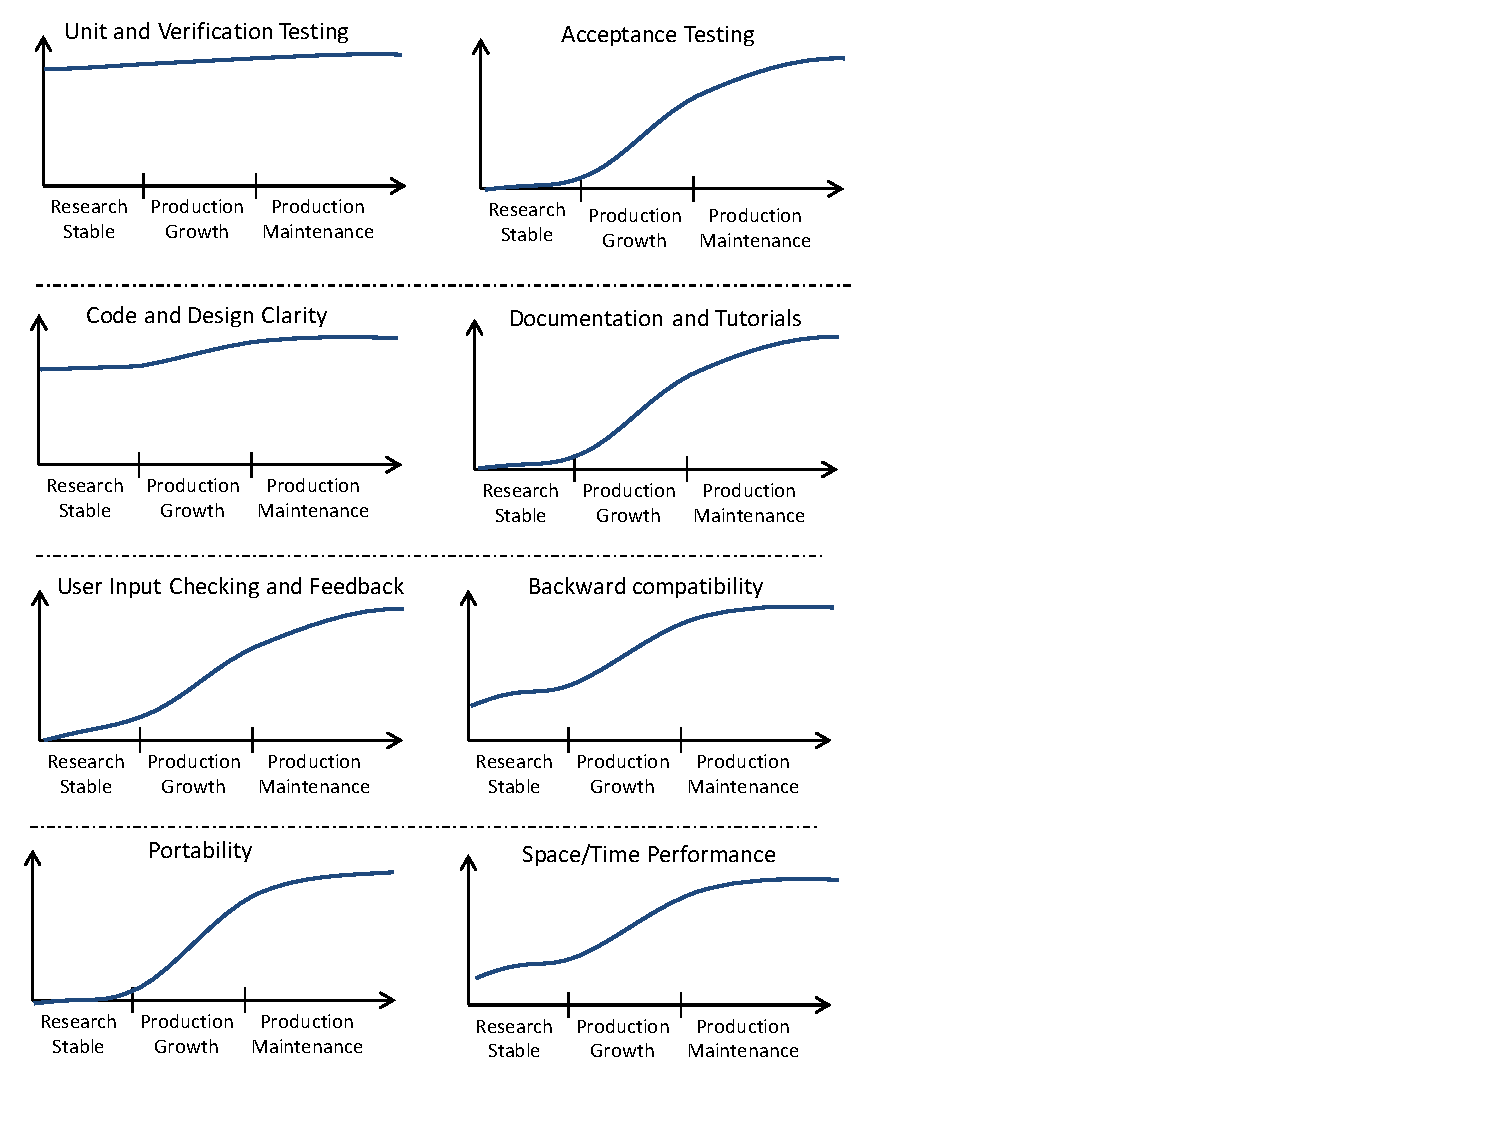
\includegraphics[trim = 0.1in 0.1in 4.0in 0.1in, scale=0.85]
{ImprovementsInDevelopmentPhases}
%}
{}\caption{Typical levels of various production quality metrics in the
different phases of the proposed Lean/Agile-consistent Trilinos
lifecycle 2.0 model.}
\label{fig:ImprovementsInDevelopmentPhases}
\end{center}
\end{figure}

Figure~\ref{fig:ImprovementsInDevelopmentPhases} shows how the
different aspects of software quality and maturity should progress
over the various phases from Research Stable through Production
Maintenance code.  What is shown is that from the very beginning,
Lean/Agile research software has a high level of unit and verification
testing (because it is developed using TDD) and maintains very clean
simple design and code base that is only improved over time.
Fundamental testing and code clarity lie at the foundation of
self-sustaining software
(Section~\ref{sec:self_sustaining_open_source_software}) and for the
transition to eventual production quality.  Acceptance testing is
related to specific end-user applications and would naturally start
out at a low level and increase as more and more users accept the
software and add acceptance tests.  Note that classical validation
testing would also be categorized as acceptance testing here; more on
that in Section~\ref{sec:risk_analysis_acceptance_testing}.

The more user-focused quality aspects of production software which
include documentation and tutorials, user input checking and feedback,
backwards compatibility, portability, and space/time performance are
improved as needed by end users and justified by various demands.  The
level of these user-oriented aspects of quality can be in very
different stages of maturity yet the software can still be considered
very good Lean/Agile software.  What differentiates Lean/Agile
Research software from Lean/Agile Production-quality software is not
the amount of testing and proof of correctness but instead is the
level of quality in these more user-focused areas.  However, when
using basic Agile development practices (including Emergent Design and
Continuous Refactoring), even ``research'' software will tend to have
a clean internal structure and have reasonably consistent user
interfaces.  These user-oriented aspects of production software will
not be overlooked as the software is productionization because they
are most directly what users see.  However, the core foundation of the
software that make it self-sustaining, which include fundamental
testing and code/design simplicity and clarity, are not directly seen
by users and these critical aspects often get overlooked as software
is ``hardened'' toward production and result in non-sustainable
software.  Therefore, the foundational elements of strong testing and
clean design and code must be established at the beginning and
maintained throughout the development of the software, even from the
first lines of research code.

It is worth mentioning that issues like version-control, automated
testing, nightly and continuous integration testing, and other basic
extremely well accepted Agile software technical practices are
already intimately woven into the Trilinos development community (see
Section~\ref{sec:trilinos_current_state}).  However, while these
policies and practices are very important, they do not directly
impact a lifecycle model except to make such a lifecycle model easier
and safer to implement.  Therefore, we will not discuss such basic
software practices and policies in this document except where needed
and instead refer the reader to the Trilinos Developers Website and
the references for details (again, see
Section~\ref{sec:trilinos_current_state}).

What is important to grasp about the new Trilinos lifecycle 2.0 model
is that steady progress is made in each of the areas (and others)
shown in Figure~\ref{fig:ImprovementsInDevelopmentPhases}.  There are
no abrupt transitional events that are required to move from one stage
to the next.  When enough of the core production quality aspects are
in place, the Trilinos team can simply declare a Trilinos package to
be in a higher (or lower) maturity level or stage.  The level of
quality in any given area or set of areas needed to achieve the next
higher maturity level is somewhat subjective and will need to be
addressed in some way when implementing this lifecycle 2.0 model.

The Exploratory code phase mentioned above is for software that is
only used to quickly experiment with different appraoches with little
concern for correctness.  The Exploratory code phase really should not
exist in a Lean/Agile consistent lifecycle model but is needed as a
catch-all for code that lacks the level of unit and verification
testing or level of design and code clarity and needed to be
considered consistent with Lean/Agile software and therefore cannot be
considered Reserach Stable code.  Such exploratory prototyping code
should be thrown away and rewritten from scratch when entering the
Research Stable phase.  Also, as mentioned above, Exploratory code
should likely not be used even for peer-reviewed published research
for journals that require reproducable research.  from the beginning
as Lean/Agile consistent Research Stable code.

The Unspecified Maturity code phase is used for software the
development teams that do not wish to participate in this lifecycle
model.

Before describing the four different phases of this new Trilinos
lifecycle model in more detail, the important concepts of
``self-sustaining software'' and ``regulated backward compatibility''
are defined in the next two sections.


%
{}\section{Self-Sustaining Open-Source Software: Defined}
\label{sec:self_sustaining_open_source_software}
%

The CSE domain is a complex and challenging domain for the development
and sustainability of high-quality software.  Many CSE projects have
development and usage lifetimes that span 10 to 30 years or more.
These projects have to port to many different platforms over their
lifetime as computing technology shifts and the software must be
augmented and changed as new and better algorithms are developed
{}\cite{HPCNeedsAToolsStrategy05}.  In such an environment, creating a
strong dependence on commercial tools and libraries can be a large
risk.  Companies are purchased and product lines go away.  (For
example, Intel purchased the KAI C++ compiler in the late 1990's and
killed it and it took years before the Intel compilers reached the
same level of quality as the KAI C++ compiler in compiling and
optimizing deeply template's C++ code.)  In addition, complex
non-commercial software produced in the U.S. national laboratories and
universities which require continuing development, maintenance and
support teams also represent a risk to long-lived CSE projects.  For
example, what happens to customer projects that adopt a complex SciDAC
software library when the funding goes away which removes the
associated supporting SciDAC-funded development and support team?

What we advocate here is that CSE software like Trilinos packages that
will be used by other CSE projects needs to be developed in such a way
as to be ``self-sustaining'' such that customer project teams could
take over the basic maintenance and support of the software for their
own use if needed.

We hereby define Self-Sustaining Software as software with the
following properties:
%
\begin{compactitem}

{}\item\textit{Open-source}: The software has a sufficiently loose
open-source license allowing the source code to be arbitrarily modified
and used and reused in a variety of contexts (including unrestricted
usage in commercial codes).

{}\item\textit{Core domain distillation document}: The software is
accompanied with a short focused high-level document describing the
purpose of the software and its core domain model
{}\cite{DomainDrivenDesign}.

{}\item\textit{Exceptionally well testing}: The current functionality
of the software and its behavior is rigorously defined and protected
with strong automated unit and verification tests.

{}\item\textit{Clean structure and code}: The internal code structure
and interfaces are clean and consistent.

{}\item\textit{Minimal controlled internal and external dependencies}:
The software has well structured internal dependencies and minimal
external upstream software dependencies and those dependencies are
carefully managed.

{}\item\textit{Properties apply recursively to upstream software}: All
of the dependent external upstream software are also themselves
self-sustaining software.

{}\item\textit{All properties are preserved under maintenance}: All
maintenance of the software maintains all of these properties of
self-sustaining software (by applying Agile/Emergent Design and
Continuous Refactoring and other good Lean/Agile software development
practices).

\end{compactitem}

The software must have a sufficiently free open-source license so that
customer projects can make needed changes to the software to suit
their needs and do critical porting work.  Alternatively, customers of
non-open-source commercial software must rely on the supplying vendor
to make needed modifications and porting which they might not be able
to do for various reasons.  Also, the open-source license must be open
enough to allow broad reuse.  For example, LGPL is okay for many
organizations but some organizations (such a commercial and even some
private for-profit companies) cannot use LGPL software.  GPL software
is also inappropriate for self-sustaining CSE software by any
reasonable measure.  However, the BSD license seems to be open enough
to allow no restrictions on use and reuse and should therefore be
preferred as the default open-source license for self-sustaining
software.

A high-level document is needed to define the scope and the high-level
goals and core domain of the software which is needed to maintain the
``conceptual integrity'' of the software~\cite{MythicalManMonth95}.
This document will be short and focused and will define the high-level
``Core Domain Model'' for the particular piece of CSE
software~\cite{DomainDrivenDesign}.  A good example of a domain model
for a multi-physics coupling package is given in {}\cite{LIMEtheory}.

As or more important than a high-level domain-model document is a
strong set of unit and verification tests.  Such tests are critical in
order to allow the software to be safely and efficiently changed to
add new features, port to new platforms, and generally refactor the
code as needed without breaking behavior or destroying backward
compatibility (see {}\cite{WorkingEffectivelyWithLegacyCode05}).  Of
course, code with strong unit and verification tests will have very
few defects (i.e.\ in Agile, there are no defects, only missing
tests).  Such a testing foundation needs to be put in place from day
one as the first lines of code are written (preferably using
Test-Drive Development (TDD) {}\cite{TDD}).  Any software lifecycle
model and process that does not include strong unit and verification
testing from the very beginning of the project is not Lean/Agile
consistent and cannot be used as the foundation for eventually
producing trusted production-quality software.

Maintaining a clean and simple internal structure of the code is
crucial for achieving self-sustaining software.  No matter how good
the unit and verification tests are, if the code is too convoluted
and/or has too many entangling dependencies and tricky behaviors, the
software will not be able to be avoidably maintained, ported to new
platforms, or changed for other purposes.  Developing software which
keeps a clean internal structure can only be done using continuous
refactoring and redesign {}\cite{XP2}.  Without applying such a
skilled and rigorous process for maintaining the software, under
maintenance and further development it will eventually die the slow
death of ``software entropy'' and become unsustainable
{}\cite{MythicalManMonth95}.  Developing software of this type
requires a high degree of skill and knowledge and places a very high
standard on CSE development teams which first create and later expand
and maintain the software.

Self-sustaining software must also carefully manage the dependencies
within itself and with its upstream software dependencies.  Within the
given software itself, if it has too many entangling dependencies and
if any particular customer does not need the majority of functionality
provided by the software, then customers are at greater risk because
the may be forced to build (and possibly port) a lot of software they
don't actually use.  For example, a given downstream customer may only
fundamentally need a few classes but if the given software has
entangling dependencies within itself, the customer may be forced to
port hundreds of thousands of lines of code just to get functionality
that should be contained in just a few thousand lines of code.  It
takes great knowledge, skill and experience to carefully partition
software and control entangling dependencies.  Similar to entangling
dependencies within a given piece of software, the more external
upstream software that is required to be downloaded, configured, and
built, the greater the risk.  In extreme cases, the shear volume of
external software packages that need to be installed before building
the given piece can massively complicate the installation and porting
of the software.  This is true no matter how portable or how easy it
is to acquire, configure, build, and install the upstream software.
The shear volume can be a significant risk.  Therefore,
self-sustaining software must carefully manage internal and external
dependencies.

Also, it is not enough for a given piece of software to satisfy the
basic properties of self-sustaining software, but it is also critical
that the dependencies of self-sustaining software also themselves be
self-sustaining software. Therefore, the definition of self-sustaining
software is recursive in nature.  For example, suppose a piece of
software is clear and well tested but has a critical dependency on a
commercial numerical library that is unique and not easy to replace.
If the vendor removes support for this critical commercial numerical
library, the downstream open-source software may become unusable and
non-portable to future platforms.

Any software that does not maintain these properties as it is ported
and maintained will slowly (or rapidly) become unsustainable which
then becomes a liability to the various downstream customer CSE
software projects.  Again, this is a high bar to define for CSE
software developers but it critical if one is serious about
sustainable large-scale CSE software integration.

Note that self-sustaining software does not necessarily have good user
documentation, really any user-oriented examples, nor necessarily
produce good error messages for invalid user input.  While these
properties of any piece of software are important for the adoption and
usage of software they do not affect the sustainability of the software
by an existing set of client projects.  The tests define the expected
behavior of the software that must be maintained (or purposefully
changed by changing the tests).


%
{}\section{Regulated Backward Compatibility}
\label{sec:regulated_backard_compatibility}
%

Backward compatibility is a central issue in Agile software
development.  The issue of regulated backward computability was
mentioned in Section~\ref{sec:life_cycle_overview} and is a critical
aspect of CSE software used by other projects.  First, the paradox of
backward computability in Agile software development is discussed and
then the official Trilinos strategy for regulated backward
compatibility is described.


%
{}\subsection{The Paradox of Backward Compatibility and Constantly
Changing Agile Software}
\label{sec:paradox_of_back_compat_agile}
%

Agile software is iteratively developed and released to customers with
very early releases preferably containing very little initial
functionality followed my many frequent releases with more and more
functionality {}\cite{AgileSoftwareDevelopment}.  All the while, the
software is constantly being refactored and refined with each new
release.  Software developed in an Agile way needs early and frequent
feedback from real customers.  Without that early and frequent
feedback from real customer usage, Agile methods fundamentally fall
apart and cannot operate.

However, most perspective customers are usually not very interested in
starting to adopt and use a piece of software that is constantly
changing with every new iterative release.  Interface changes in
aggressively developed software break customer code and require the
downstream developers to constantly be chasing changes, and dealing
with broken builds and changing behavior.  Most customers would rather
wait until the perspective software ``stabilizes'' before deciding to
start using the software (and therefore start giving feedback).  But
here in lies the paradox; Agile developed software cannot stabilize
its interfaces and behavior unless customers use the software and give
feedback after many iterations of releases but customers do not want
to adopt software that is constantly changing.

So if customers do not want to use software that is constantly
changing and Agile developed software cannot stabilize unless its gets
feedback from customer usage, how can Agile development working?  How
can we actually develop Agile software without placing an unreasonable
burden on customers?  The answer is to carefully manage changes in
Agile developed software interfaces and behavior and smooth the
transition for customers to make upgrades of iterative (or continuous)
releases as easy, safe, and painless as possible.  The way we do that
is to adopt a rigorous set of policies and practices for
{}\textit{regulated backward compatibility} (to be defined in
Section~\ref{sec:defined_reg_back_compat}).


%
{}\subsection{The Need for Backward Compatibility}
\label{sec:need_for_back_compat}
%

Backward compatibility is critical for safe upgrades of new releases
of software and for the composability and compatibility of different
software collections.  If every new release of a piece of software
breaks backward compatibility, it discourages users from depending on
the software and/or discourages accepting new releases.  In the case
of CI, if a package constantly is breaking backward compatibility, then
downstream packages must constantly be updated to keep up, making for
a difficult and inefficient development process.  In the case of
composability of software through releases, some backward
compatibility is critical to allow for different collections of
software to be integrated.

To demonstrate the critical need for backward compatibility for
allowing the composibility of software, consider the scenario shown in
Figure~\ref{fig:XyceSierraVtkTrilinosCompatibility}.  This scenario
shows three different software collections that depend on Trilinos and
depend on each other.  Here, Xyce version J+1 is released which is
tested and certified against Trilinos version X.  After that, Trilinos
puts out release X+1.  This is followed by the release of VTK version
M+1 which is tested and certified against Trilinos X+1.  Finally,
SIERRA version Y+1 is released which is tested and certified against
its own local snapshot of Trilinos called Trilinos version SIERRA Y+1.
Here SIERRA has optional dependencies on Xyce and VTK for which it uses
static releases.  In this scenario, what version of Trilinos can be
used that is compatible with Xyce J+1, VTK M+1 and SIERRA Y+1?  If
each Trilinos release breaks backward compatibility with each previous
release in a non-trivial way, then there is no single version of
Trilinos in existence that will allow the integration of Xyce J+1, VTK
M+1 and SIERRA Y+1 in the same statically linked executable and
trying to mix in multiple library versions of Trilinos will result in
link-time errors\footnote{When using dynamic linking, it is possible
to mix multiple versions of a library in the same executable so it is
possible to use non-backward compatible versions of a library in a
dynamically linked program.  However, may of the high-end HPC
platforms only allow static linking so relying on dynamic linking to
address incompatible library versions is not a viable solution for CSE
HPC software.}.

\begin{figure}
\begin{center}
%\fbox{
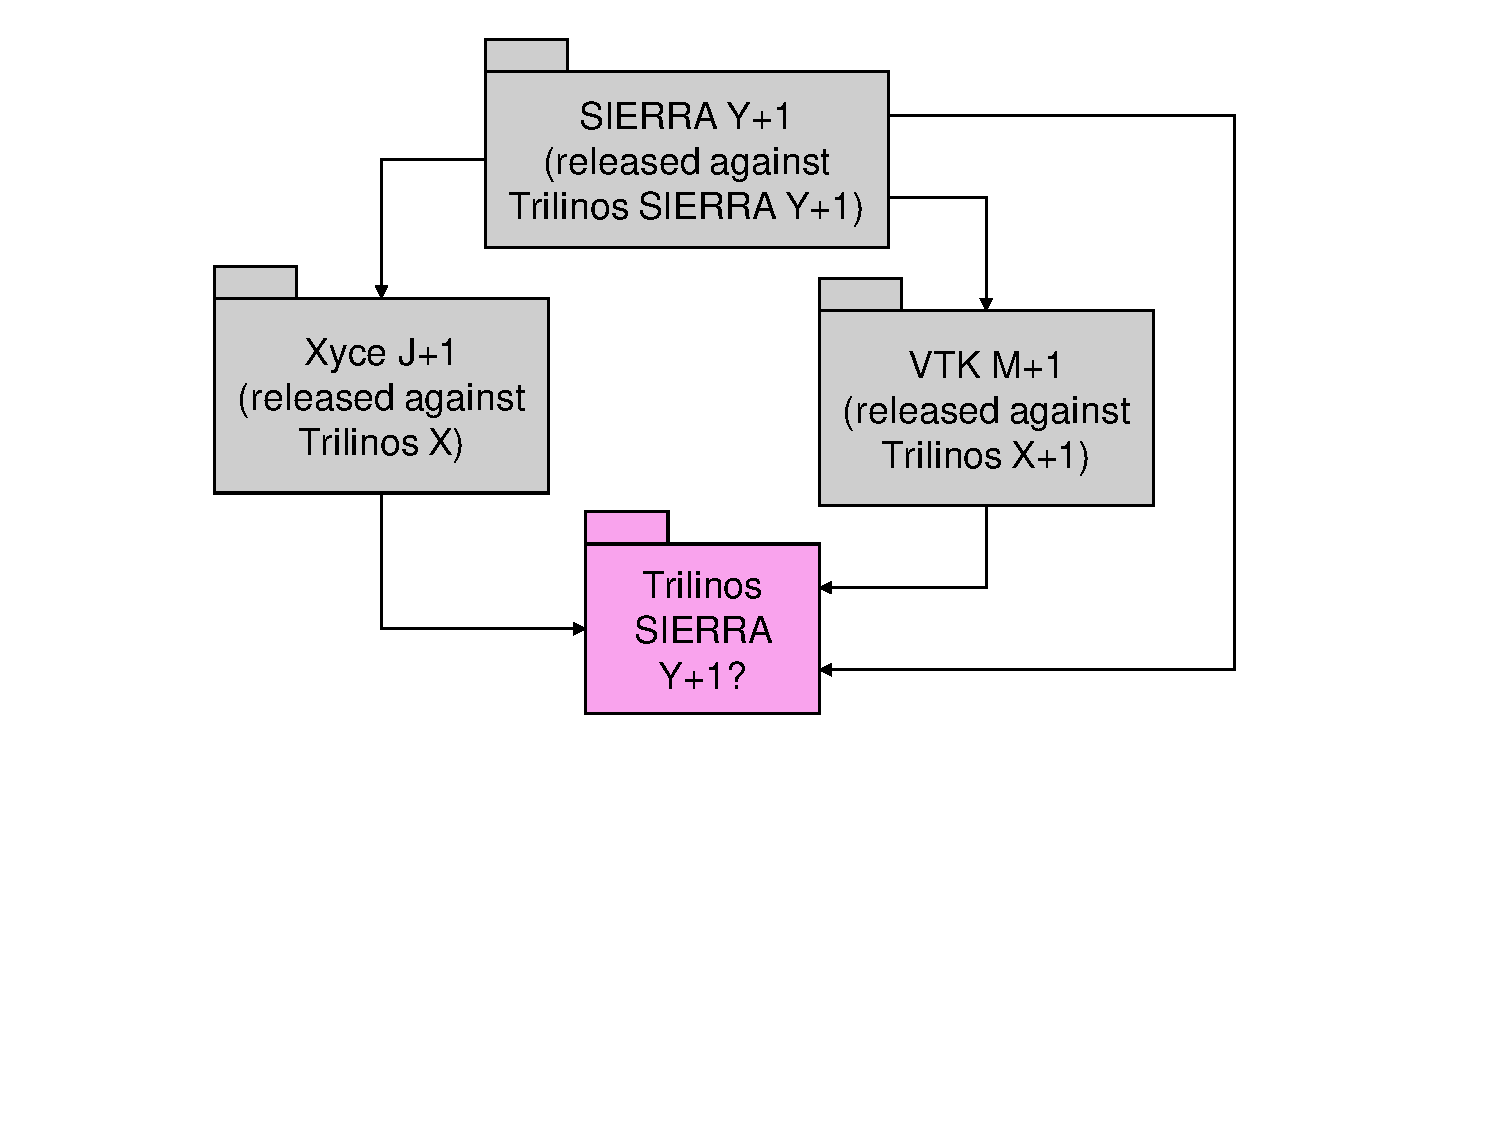
\includegraphics[trim = 1.0in 2.7in 1.0in 0.2in, scale=0.55]
{XyceSierraVtkTrilinosCompatibility}
%}
\caption{
Example that demonstrates of the need for backward compatibility among
multiple releases of Trilinos and customer applications.}
\label{fig:XyceSierraVtkTrilinosCompatibility}
\end{center}
\end{figure}

However, if Trilinos releases maintain rigorous backward compatibility
between releases Trilinos X through Trilinos SIERRA Y+1, then the
integration and release scenario shown in
Figure~\ref{fig:XyceSierraVtkTrilinosCompatibility} is easily
achieved.

Without sufficient backward compatibility, such integration scenarios
becomes very difficult and would otherwise require that the (static)
releases of Xyce J+1 and VTK M+1 be updated to Trilinos version SIERRA
Y+1.  Such upgrades would be done, typically, without the aid of the
core Xyce or VTK development teams and performing these upgrades could
be expensive and risky.  All of these difficulties, risks, cost, and
uncertainty in developing and releasing such downstream software all
but go away if the upstream library (Trilinos in this case) maintains
backward compatibility across all of the needed versions.


%
{}\subsection{The Cost of Maintaining Backward Compatibility}
\label{sec:costs_of_back_compat}
%

While maintaining some backward compatibility is a critical
requirement for large-scale development and software integration (in
CI or through releases) as described above, maintaining backward
compatibility also comes with potentially high costs over a long lived
project.  The main costs of maintaining backward compatibility are the
extra testing needed to prove backward compatibility and the cost of
the accumulation of technical dept that occurs because of the
inability or added difficulties to refactor software or to not allow
for better/safer designs and code.

As new features are developed and new interfaces are created,
maintaining backward compatibility requires keeping older versions of
classes and functions around with the old behavior.  Keeping around the
old interfaces and functionality bloats the code base and requires
more code to build and more tests to run and maintain.  This overhead
of extra code to maintain, build, and test taxes the entire
development effort.  Dropping backward compatibility, however, allows
for deleting old obsolete software and tests and makes the entire
development effort run faster and more efficiently.

Also, the extra cost in maintaining old interfaces and behavior as new
behavior is created discourages the creation of or refactoring to new
interfaces and behaviors.  Instead of changing existing interfaces
(which would break backward compatibility), developers are drawn to
keep the same interfaces in place and then put in ``work-arounds'' to
add new behavior.  Often these tweaks are not done in a clean way and
the resulting software becomes messier lacking of consistent
structure.  This tendency of software under subsequent releases and
modifications to loose its internal structure was refereed to as
``software entropy'' in {}\cite{MythicalManMonth95}.  Without constant
refactoring to clean up the interfaces and design of the software
(which often breaks backward compatibility), such software dies a slow
death of rising ``technical debt''
{}\cite{ImplementingLeanSoftwareDevelopment}.  However, when backward
compatibility is not maintained, then the software can be freely
refactored to maintain ``conceptual integrity''
{}\cite{MythicalManMonth95}.

Therefore, while it is easy to see the critical need for maintaining
some backward compatibility as described in
Section~\ref{sec:need_for_back_compat}, we have also acknowledged that
maintaining backward compatibility over a long lived piece of software
can impart significant extra cost and/or significantly increase the
``software entropy'' and ``technical debt'' of the software that will
eventually make the software unable to continue to be changed from a
cost/benefit point of view.  In other words, the code will become
unsustainable (i.e.\ not self-sustaining) software.

%
{}\subsection{Regulated Backward Compatibility: Defined}
\label{sec:defined_reg_back_compat}
%

In order to balance the need and benefits of maintaining backward
compatibility described in Section~\ref{sec:need_for_back_compat}
against the costs of maintaining backward compatibility described in
Section~\ref{sec:costs_of_back_compat}, we here define a compromised
approach called {}\textit{Regulated Backward Compatibility}.  In this
approach, sufficient windows of backward compatibility are maintained
in order to achieve most of the benefits of maintaining backward
compatibility but backward compatibility can be dropped periodically
to avoid the accumulation of technical debt and extra testing related
to maintaining backward compatibility.

The Trilinos approach for implementing regulated backward
compatibility is inherent in the Trilinos version numbering scheme
{}\textbf{X.Y.X} where
%
\begin{compactitem}
%
{}\item\textbf{X} defines a backward compatible set of releases,
%
{}\item\textbf{Y} is the major release (taken off of the master
branch) in backward compatible set X, and
%
{}\item\textbf{Z} is the minor release off the release branch X.Y.
%
\end{compactitem}

\begin{wrapfigure}{r}{0.5\textwidth}
\begin{center}
\fbox{
\begin{minipage}[b]{0.45\textwidth}
{}\textbf{Side Node:} A special exception to the even/odd numbering
method for release/development versions is made when moving from X to
X+1 (e.g., 11.6 to 12.0 releases).  Once the last major release in the
set X.Y is branched (e.g., 11.6), then the version of the development
sources are immedately changed to X+1.0 (e.g., 12.0) instead of X.Y+1
or X+1.-1.  This convention allows downstream customer code to use
ifdef logic based the unsigned integer version number in
{}\ttt{Trilinos\_version.h} to show the major switch in backward
compatibility sets for those that are building against the development
version of Trilinos but yet does not require support for negative
version numbers.
\end{minipage}
} %fbox
\end{center}
\end{wrapfigure}

The numbers Y and Z use even numbers for releases and odd numbers for
development versions between releases.  This release number X.Y.Z is
given in integer form in macros in the configured header file
{}\ttt{Trilinos\_version.h}.  This numbering scheme X.Y.Z with
even/odd numbers allows client code to manage different versions of
Trilinos just by using pre-processor logic.

To demonstrate how the backward compatibility is managed, consider the
release time-line with backward compatibility indicators shown in
Figure~\ref{fig:BackwardCompatibilityTimeline}.  This scenario shows
four major releases in the backward compatible set 11.Y (11.0, 11.2,
11.4, and 11.6).  In the set 11.Y, each version is compatible with all
of the prior versions.  For example, 11.6 is compatible with all of
the previous versions 11.0, 11.2, and 11.4.  However, the transition
from 11.6 to 12.0 drops guarantees of backward compatibility between
the two versions.  Section~\ref{sec:details_reg_back_compat} describes
how this transition to the next backward compatible set is handled.

\begin{figure}
\begin{center}
%\fbox{
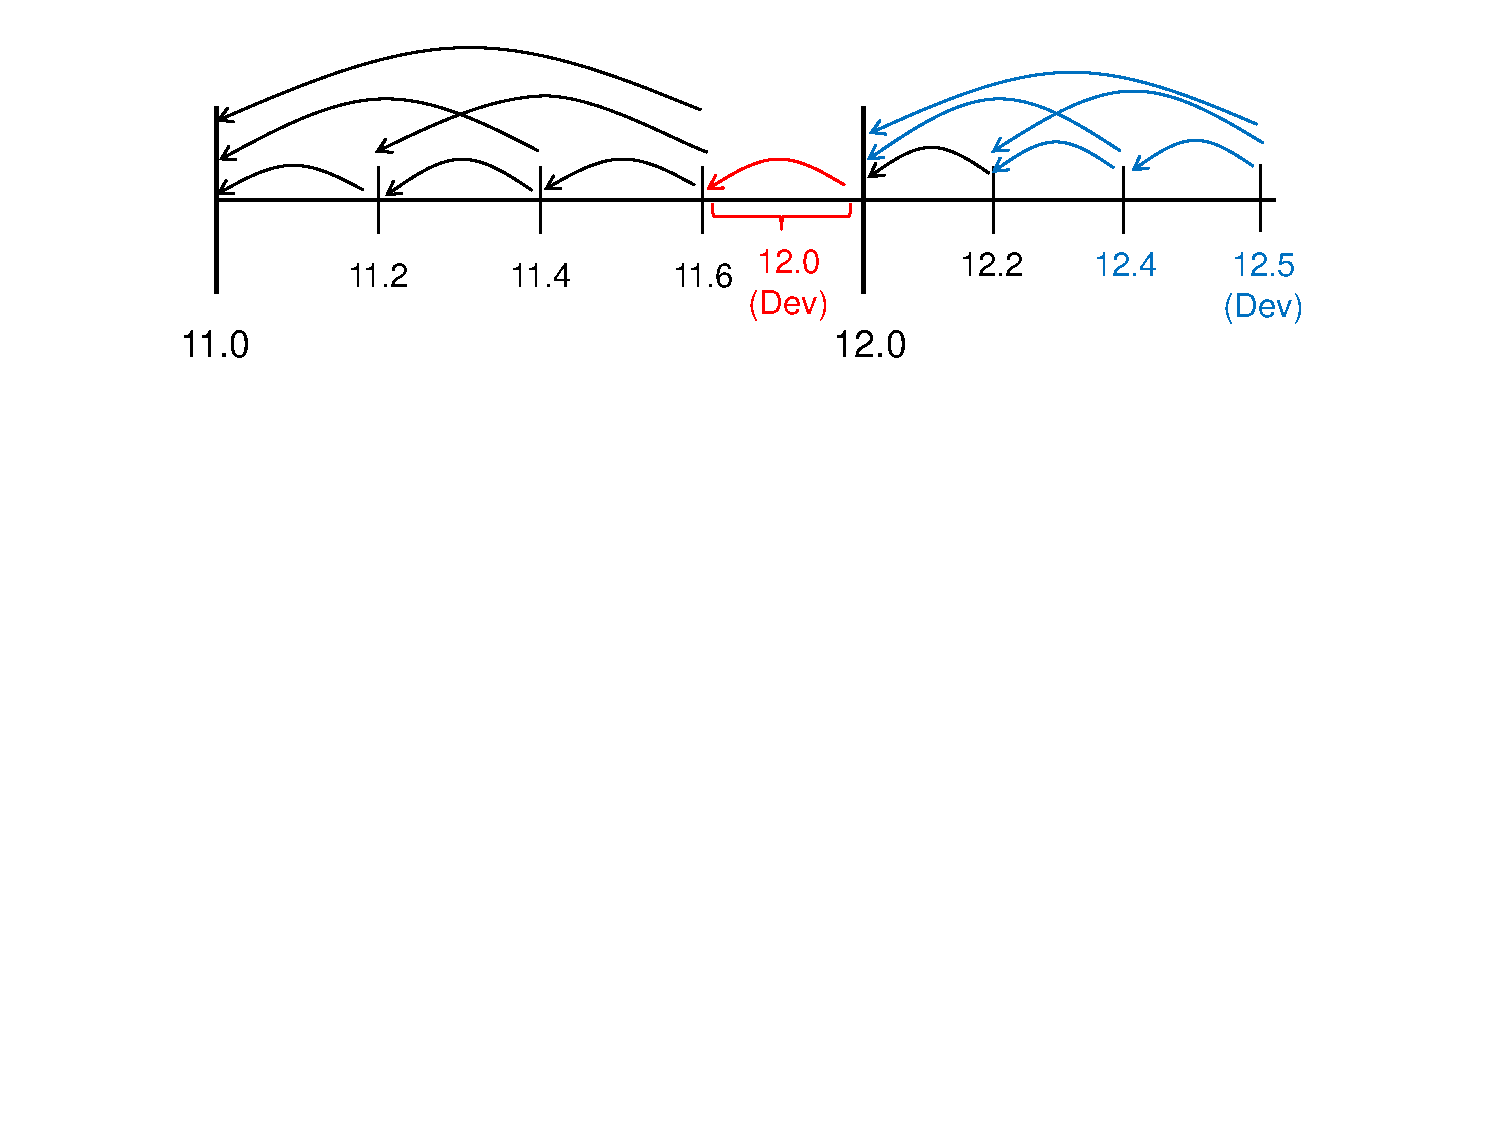
\includegraphics[trim = 1.0in 5.0in 1.0in 0.2in, scale=0.55]
{BackwardCompatibilityTimeline}
%}
{}\caption{Regulated backward compatibility release time-line.}
\label{fig:BackwardCompatibilityTimeline}
\end{center}
\end{figure}

With this approach, the balance between maintaining backward
compatibility and minimizing the cost of maintaining backward
compatibility is controlled by how many releases X.Y are in a
backward compatible set X.  Let $N$ be the number of releases X.Y in
the backward compatible set X.  If $N$ is smaller, then less effort is
expended on maintaining backward compatibility but might result in
more problems with customer upgrades.  For example, if Trilinos only
had two major releases X.0 and X.2 in a backward compatible set X, it
would be difficult to accommodate a usage scenario with three
dependent customer application codes as shown in
Figure~\ref{fig:XyceSierraVtkTrilinosCompatibility}.  Alternatively,
if $N$ is high then backward compatibility is maintained for long
periods of time over many releases.  This enables a number of usage
and integration scenarios for downstream customer codes but the cost
of maintaining backward compatibility may become very large.


%
{}\subsection{Regulated Backward Compatibility: Details}
\label{sec:details_reg_back_compat}
%

There are two critical aspects to the implementation of regulated
backward compatibility that must be discussed: backward compatibility
testing, and the handling of dropping of backward compatibility.

Within a backward compatible set X, it is not enough to simply try or
desire to maintain backward compatibility, it must be tested.  Within a
backward compatible set X, testing must be performed to ensure that
each subsequent version X.Y is backward compatible (to some level)
with the previous versions X.Y-1, X.Y-2, etc.  Testing of backward
compatibility is accomplished in Trilinos by building a suite of
user-oriented tests for an older version of Trilinos (e.g., 12.0 or
12.2) against the installed headers and libraries of a newer version
of Trilinos (i.e.\ the current release 12.4 and development version
12.5 in Figure~\ref{fig:BackwardCompatibilityTimeline}).  Note that
backward compatibility is only actively tested for the current release
(e.g., 12.4) and the current development version (e.g., 12.5) since
the older releases should all be static.  For example, for the
scenario shown in Figure~\ref{fig:BackwardCompatibilityTimeline},
Trilinos release 12.4 would be tested against 12.2 and 12.0 and
Trilinos development version 12.5 would be tested against 12.4, 12.2,
and 12.0.  Therefore, the amount of backward compatibility testing is
proportional to the number of releases in a backward compatibility
set.  If $N$ is the number of releases in the backward compatible set
X, then $2 N-1$ backward compatibility builds must be performed on a
regular (nightly) basis.  While not perfect, this approach provides
developers and users some assurance that backward compatibility is
being maintained.

Note that by using this testing approach, the level of confidence in
the maintenance of backward compatibility is only as good as the quality
of the user-oriented tests that are built and run.  This test suite
should likely contain the entire verification and acceptance test
suites if possible.  The unit test suite could also be included in the
set of tests but that might overly constrain backward compatibility
but on the other hand would strengthen the testing of backward
compatibility.

Note that the number of backward compatible releases determines how
many nested collections downstream of software can be kept integrated,
assuming they use the Punctuated Releases approach to software
integration {}\cite{SoftwareIntegrationforCSE09} where each
application software just builds against a static release of Trilinos
and other external software.

For example, if Trilinos provides backward compatibility for three
contiguous releases, it allows for up to three nested client
application codes to depend on each other and Trilinos, as shown in
Figure~\ref{fig:ThreeAppsDependingOnTrilinos}.  The releases of the
three applications are depicted in
Figure~\ref{fig:ThreeAppsDependingOnTrilinosReleases}.  Here new
releases for App1 K+1, App2 M+1, and App3 J+1 are put out against
three consecutive releases of Trilinos such that the final release
App3 J+1 (against App2 M+1, App1 K+1 and Trilinos X+3) has the most
recent versions of Trilinos and each of its upstream dependent Apps.
Therefore, if there are only $N$ consecutive releases of Trilinos,
then at most only $N$ sets of nested applications can be supported in
the most general case (e.e.\ where each upgrades the most recent
Trilinos release).  And this can be done without any coordination
between the Trilinos and the downstream development teams.  If
backward compatibility is not maintained for enough consecutive
releases, then some amount of coordination and negation are needed
between the Trilinos and the various App development teams.  This type
of coordination is neither desirable nor practical in many cases.

\begin{figure}[p]
\begin{center}
%\fbox{
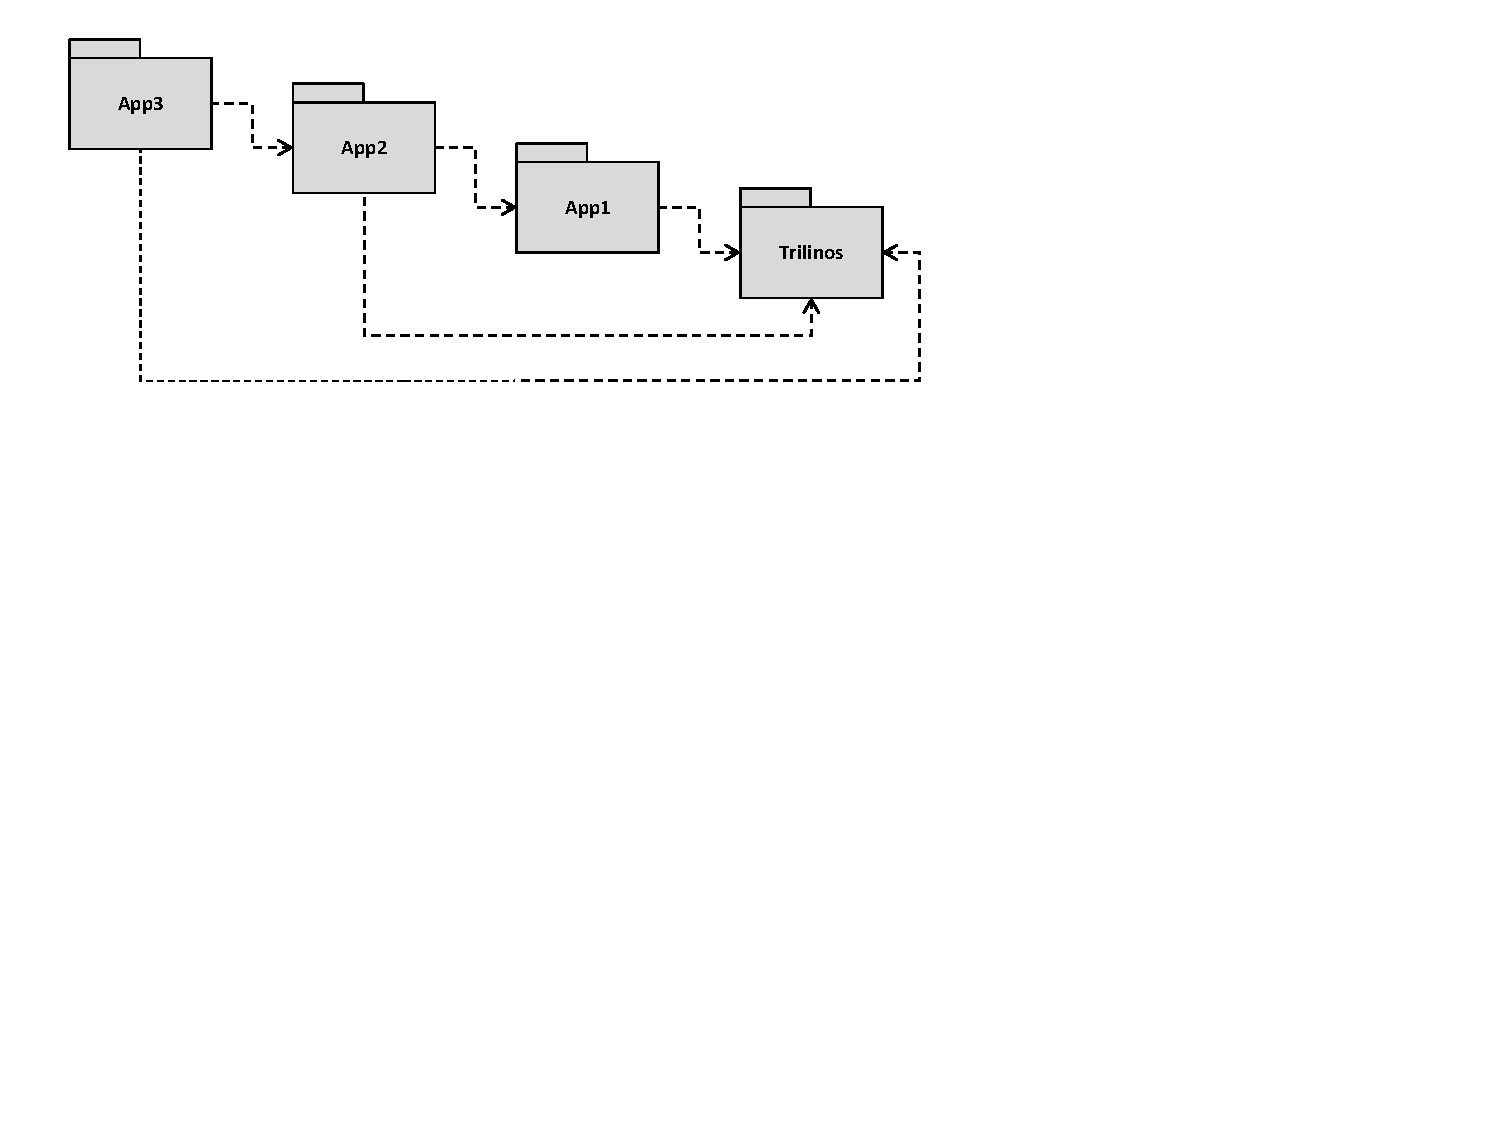
\includegraphics[trim = 0.2in 4.8in 3.6in 0.1in, scale=0.75]
{ThreeAppsDependingOnTrilinos}
%}
{}\caption{An example of a chain of three applications that depend on
Trilinos and each other linearly.}
\label{fig:ThreeAppsDependingOnTrilinos}
\end{center}
\end{figure}

\begin{figure}[p]
\begin{center}
%\fbox{
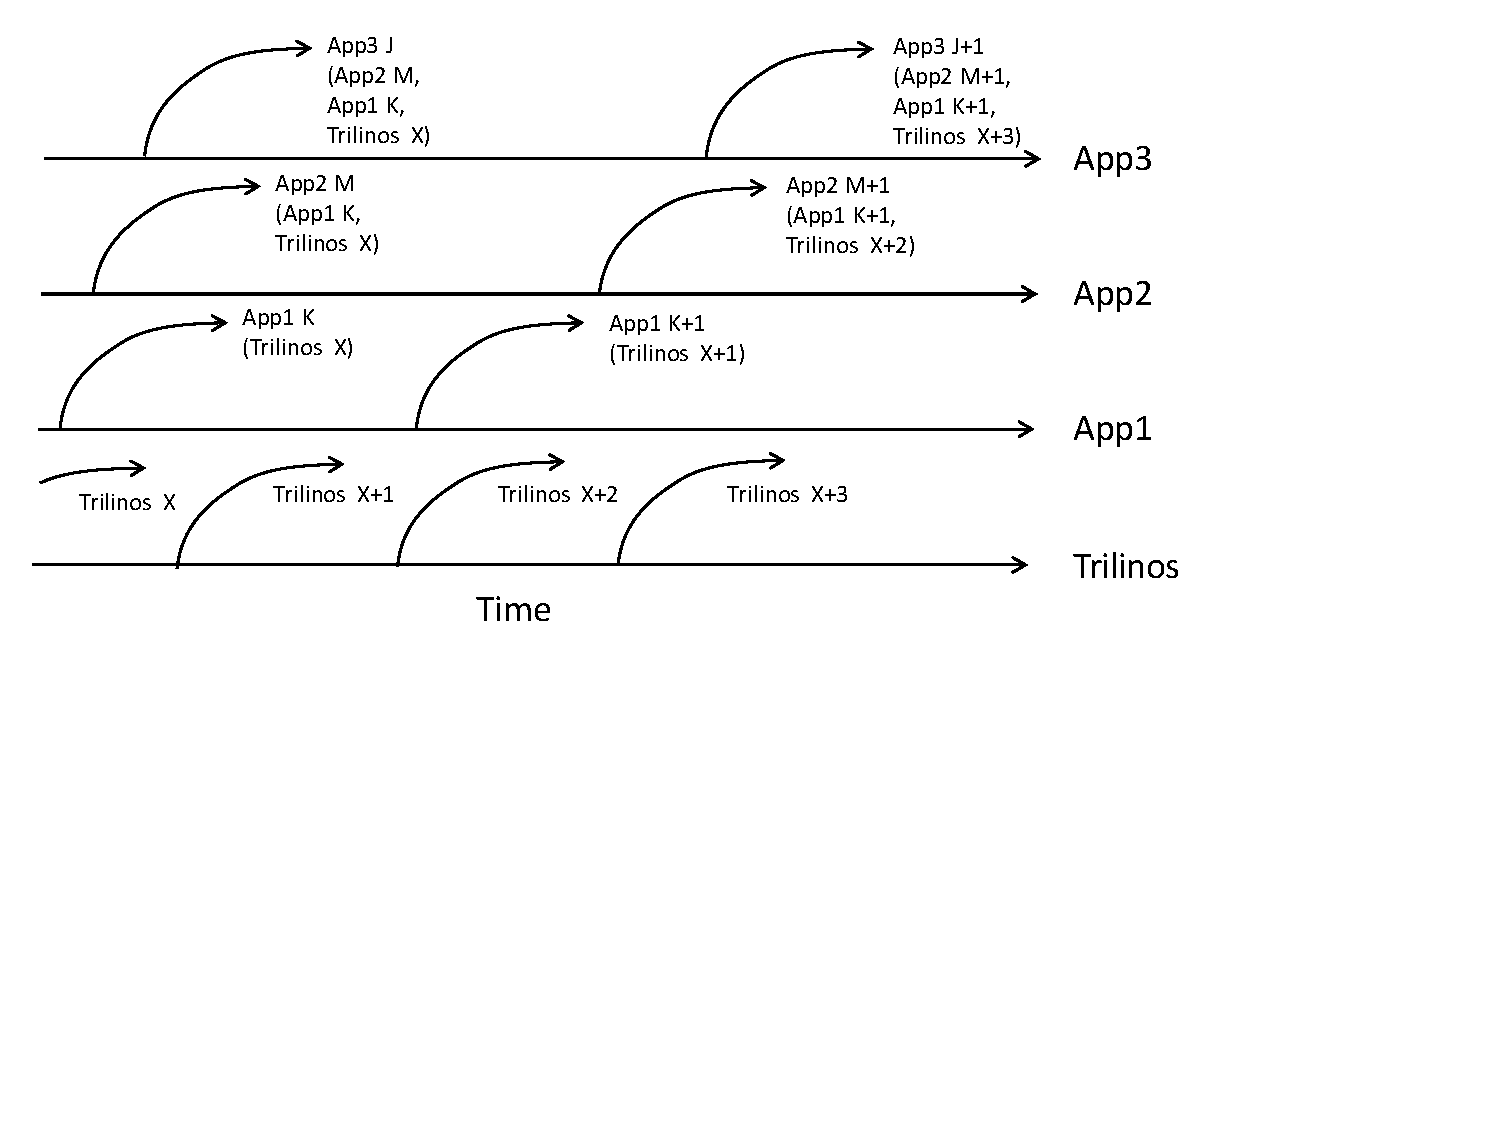
\includegraphics[trim = 0.2in 3.2in 2.2in 0.1in, scale=0.75]
{ThreeAppsDependingOnTrilinosReleases}
%}
{}\caption{An example of the releases of chain of three applications
that depend on Trilinos and each other linearly.}
\label{fig:ThreeAppsDependingOnTrilinosReleases}
\end{center}
\end{figure}

The second and more challenging aspect to implementing regulated
backward compatibility is handling the dropping of backward
compatibility between backward compatible sets X and X+1 while easing
the transition for downstream users and development teams.  Simply
putting out a release that breaks backward compatibility and breaks
user code without any warning or means to help them upgrade their code
is irresponsible and counterproductive.  Even worse is when changes in
backward compatibility allow user code to still build but fails in
subtle ways which is even more unacceptable.

So how is the transition between backward compatible sets (e.g., from
11.6 to 12.0) managed?  Here are some guidelines for managing the
breaking backward compatibility when transitioning between backward
compatible sets X and X+1:

\begin{compactitem}

{}\item\textit{Prepare users for the break in backward compatibility}:
Try to to provide some preparation for breaking backward compatibility
in previous releases.  The best way to do this is to mark code as
``deprecated''.  The GCC and Intel C++ compilers support a
{}\ttt{\_\_deprecated\_\_} property that can provide compile-time
deprecated warnings for classes and functions.  There are many
strategies for appropriately deprecating code to allow users a means
to perform smooth transitions to new functionality before backward
compatibility is dropped.

{}\item\textit{Fail big and hard when backward compatibility is
dropped}: When breaking backward compatibility, client code should
break in an obvious way.  Ideally, non-upgraded client code should not
even compile and the compile errors should be as obvious as possible.
If compile errors are not possible, link-time errors would be the next
best alternative.  If compile or link errors are not possible, then
run-time errors should be generated with good error messages helping
the user to know what needs to be changed.

{}\item\textit{Provide for safe straightforward upgrades}: When
breaking backward compatibility, try to provide the user an easy and
error-proof approach to upgrade their code.  For example, when
changing the name of a set of classes and functions, provide a
sed-like script that the user can run on their code to preform the
name changes.  This can be difficult for raw class and function names.
However, for globally unique identifiers (like C function and macro
names) these sed-like scripts are very safe.

\end{compactitem}

Here are some guidelines for deprecating functionality to prepare
users and downstream developers to upgrade their code:

\begin{compactitem}

{}\item\textit{Deprecate classes and functions using the standard
{}\ttt{<UCPACAKGENAME>\_DEPRECATED} macro}: This macro expands to the
GCC {}\texttt{\_\_deprecated\_\_} attribute when Trilinos is
configured with {}\ttt{Trilinos\_SHOW\_DEPRECATED\_WARNINGS = ON}.

{}\item\textit{Deprecate macros by calling dummy deprecated functions
using the standard {}\ttt{<UCPACAKGENAME>\_DEPRECATED} macro}: Any
macro that can work by creating a nested scope as {}\ttt{\{
SomeDeprecatedFunction(); ... \}} can use this approach.  Other macros
that can't create a nested scope to call a deprecated function like
this are more problematic.

{}\item\textit{Deprecate old class names using deprecated typedefs or
macro defines}: When changing the names of classes, keep the old names
using safe deprecated typedefs for non-templated classes.  However,
for templated classes, C++98 does not allow the use of typedefs and
therefore macros defines must be used to keep the old class names in a
way that works with templates.  These macros, however, cannot be
deprecated (but the old deprecated header file they are in can be, see
below).

{}\item\textit{Deprecate header files by inserting protected
{}\texttt{\#warning} directives}: A header file would be deprecated,
for example, when changing the name of a class which would therefore
require changing the name of its header and source files.

\end{compactitem}

Examples of the usage of the above deprecation approaches can be found
throughout Trilinos.  By carefully deprecating code, downstream users
and developers can safely and incrementally refactor their code to
remove use of deprecated features.  This refactoring to upgrade code
be done in a relaxed and safe way since the changes can usually be
made in small batches which include rerunning their test suites.  Over
time, downstream code developers can remove all deprecated warnings
which will allow them to build and run successfully after backward
compatibility is dropped.

In the ideal case, the transition from X.Y to X+1.0 (e.g., 11.Y to
12.0) would be accomplished by simply having the downstream code build
against the last compatible release in the set X.Y (e.g., 11.6),
remove all of the deprecated warnings (either manually or through
provided sed-like scripts), and then transition to X+1.0 with no
further changes.  While this is the safest and most attractive approach
for dealing with backward compatibility for downstream users and
developers, there are some types of changes that are very hard to
manage in this way.  For example, if it is desired to change the
naming of a large number of templated C++ classes, it may be more
desirable to instead wait until the last release in X is put out
(e.g., 11.6) and then create a sed-like script to change a bunch of
class names and file names all at once.  This sed script would be run
on the Trilinos code base right away and all downstream software
projects that do Almost Continuous Integration
{}\cite{SoftwareIntegrationforCSE09} with Trilinos.  This would also
work well for downstream projects that do Punctuated Upgrades
{}\cite{SoftwareIntegrationforCSE09} of Trilinos releases.  As soon as
they transitioned to Trilinos 12.0, for instance, they would run the
provided sed-like upgrade scripts and be done (except for perhaps a
little manual cleanup).  However, downstream customer codes that do
Release and Dev Daily Integration {}\cite{SoftwareIntegrationforCSE09}
would have a harder time because their code base could not be
simultaneously compatible with both 11.6 and 12.0.  In this case, they
may need to drop building against either 11.6 or the development
version leading to 12.0 (their choice will depend on their particular
needs and constraints).


%
{}\section{Detailed Discussion of the Proposed Lifecycle Stages}
\label{sec:detained_lifecycle_stages}
%

Now that the four different lifecycle phases have been introduced and
the concepts of self-sufficient software and regulated backward
compatibility have been described, the four different lifecycle phases
are discussed in more detail.


%
{}\subsection{Exploritory}
\label{sec:exploratory_code}
%

As mentioned in Section~\ref{sec:life_cycle_overview}, the Exploratory
code stage is a place-holder for any research software that has not
been developed in a Lean/Agile consistent way and is not an
appropriate direct foundation for later development of
production-quality software.  For example, software with very low
coverage of testing can likely not be considered to be Research Stable
software.  Howver, such software will be written for rapid prototyping
purposes.

The Exploratory code phase and lax practices associated with it should
only be used for software and algorithms that have a low probability
of success and therefore of later being considered for
productionzation.  Otherwise, if the appraoches or aglorithms have a
high probability of being successful and for being later
productionized, it will be overall more productive and more efficient
to implement the software from the very beginning as Research Stable
software as described below.  Otherwise, if the algorithms and
appraoches in Exploratory software prove to be attractive for
productionalization, new software should be written from scratch using
the practicies described for Research Stable software below.


%
{}\subsection{Research Stable}
\label{sec:research_stable_code}
%

The Research Stable stage is the initial stage for Lean/Agile
consistent research software development.  The goal in this stage is
to experiment with various approaches, generate credible publishable
results, and form the foundation for the probable future
productionization of the software.

All code in this stage should be written using Test-Driven Development
(TDD) which will yield nearly 100\% line coverage with minimal extra
effort.  This is depicted in
Figure~\ref{fig:ImprovementsInDevelopmentPhases} with ``Unit and
Verification Testing'' starting at a high level and staying high.
This level of testing might seem excessive to some not accustomed to
the TDD software development process but even from a research
perspective, these tests can help to avoid defects that would
otherwise taint research results.  Another important Lean/Agile
consistent development practice is to keep the code base very clean
and clear, avoiding unnecessary complexity.  Once good design and
refactoring skills have been acquired, maintaining a clean code base is
easier than crafting a messy/complex code.  This is also depicted in
Figure~\ref{fig:ImprovementsInDevelopmentPhases} by having ``Code and
Design Clarity'' start out high and stay fairly high.  Having a clean
code base is also critical for just research software in order to
verify that the algorithms and approaches described in a research
publication are indeed what are implemented in the code.  Also, as
more journals start to require the submitting and review of source code
and test inputs used to generate published results, strong unit and
verification tests and a clean code base allow for a much easier
review and greater chance of having a paper accepted.  In addition to
being important from just a verifiable reproducible research
perspective, excellent unit and verification tests and a clean and
clear code base form a critical foundation for creating
self-sustaining software (see
Section~\ref{sec:self_sustaining_open_source_software}) and providing
a foundation for possible later productionization of the code.

While Lean/Agile Research Stable software needs to have high-quality
unit \& verification testing and clean code, it need not have much of
if any documentation, it can have very little error checking of
invalid user input and no feedback in case of incorrect input (it can
just assert() and die), and it may not have any acceptance testing
(because there are no real customers).  While addressing these issues
is critical for high-quality production software, they are of little
use for pure research software (that is used by only the core
developers or very friendly and intimate users).  In addition,
Research Stable software need not maintain any backward compatibility
at all if there are no down-stream customers (and there should not be
too many down-stream customers for a pure research code).  Any
downstream customers that would be affected by a break in backward
compatibility should be readily accessible to upgrade when non-backward
compatible changes are made.

Finally, Research Stable software really only needs to build and run
successfully on the primary Trilinos development platform (currently
GCC 4.5+).  While this might sound like a bad way to develop software
that is being targed for possible later productionization, consider
that the Trilinos CMake build system automatically inserts strong
options into every build (see
Section~\ref{sec:trilinos_current_state}), even for Exploratory and
Research Stable code.  Extensive experience has shown that C++ code
that builds clean of warnings with these strong compiler warning flags
that has a good test suite (which Research Stable software does by
definition) typically has few serious problems when porting to other
platforms.  Therefore, portability to other platforms is not
considered a concern for Research Stable software in order to enter
the next phase, the Production Growth phase.

The last issue to consider in the lifecycle of software is space/time
performance.  For most research-based software, algorithmic properties
are the primary concern, not raw performance.  In addition, premature
code optimization efforts can greatly damage the clean design and
layout of the code.  Therefore, code optimization to improve
space/time performance metrics should only be considered in the
Research Stable phase when the focus of the research is on low-level
performance.  Otherwise, the focus should be on writing clean well
tested software.

If the appraoches or algorithms being researched have a low
probability of being successful, being submitted for publication, or
being considered for later productionalization, then it may be more
efficient to develop the software as Exploratory software as described
above.


%
{}\subsection{Production Growth}
%

After the algorithms in a piece of software have been sufficiently
proven in the Research Stable phase, the software is a candidate to
pursue for productionization.  Since the Research Stable code already
has excellent unit and verification testing and has a clean design and
source code, it is immediately ready to enter the Production Growth
phase.

\begin{wrapfigure}{r}{0.5\textwidth}
\begin{center}
\fbox{
\begin{minipage}[b]{0.45\textwidth}
{}\textbf{Side Note:} It is also possible to take Exploratory software
and turn it into Research Stable software that can seed the Production
Growth phase but it would require a large refactoring effort driven by
an intense unit and verification test development effort.  The large
cost needed to get Exploratory code to the standard of quality needed
for Research Stable code (the precondition for entering the Production
Growth phase) is usually not undertaken and therefore software that is
not developed from the beginning with strong testing with continuous
refactoring to maintain clear design and code typically never achieves
the properties necessary for self-sustaining software.  Therefore,
again, Exploratory software should likely be thrown away and rewritten
from scratch as Research Stable software.
\end{minipage}
} %fbox
\end{center}
\end{wrapfigure}

When software enters the Production Growth phase, the purpose is to
start adding those features needed to make the software more usable
for downstream clients and add functionality needed to support their
mission.  However, while a primary focus is on starting to improve the
production quality of the software, the software can still be used for
new research to some extent but the overhead of doing research in the
code base will become larger and larger as the software becomes more
productionized (and has to maintain better backward compatibility,
needs better documentation, etc.).  Continued research can be
conducted in related subpackges to minimize the impact on the body of
software under consideration that is beginning productionized.

In the Production Growth phase, the user-oriented elements start to
get fleshed out, as depicted in
Figure~\ref{fig:ImprovementsInDevelopmentPhases}, including adding
documentation and tutorials, adding more tests for boundary conditions
for invalid user input (and improving error messages that are
generated), and starting to become increasingly more careful about
maintaining backward compatibility.  All the while new features are
developed and functionality changes, the unit and verification testing
is continued and even expanded slightly to cover more boundary cases
and other scenarios.  At the same time, the code is continually being
refactored to keep the design simple and the code layout clean and
understandable.  This is done while maintaining backward compatibility
by deprecating features thereby giving downstream developers the
chance to safely upgrade their code to keep up with the changes (see
Section~\ref{sec:details_reg_back_compat}).

This is also the stage where more serious customers can start to
depend on the software because they know that backward compatibility
will be handled more carefully and the development team will be trying
to improve documentation, error checking and reporting, and will be
integrating acceptance tests that the customer develops with them.  At
the beginning of the Production Growth phase, backward compatibility
may not be maintained very well and downstream developers may have a
hard time keeping up with the changes.  However, quickly the upstream
team should start doing a better job of deprecating features and
smoothing the transition for downstream customer code and developers.
The relationship with downstream customers is greatly facilitated if
Almost Continuous Integration {}\cite{SoftwareIntegrationforCSE09} is
used where deprecated features are seen right away and breaks in
backward compatibility and caught and addressed in short order.

As more customers are added, more platforms will need to be supported
beyond just the single primary development platform.  Therefore, the
Production Growth phase will see the portability of the software
radially increased.  Likewise, in order to entice new customers or to
even make the software viable to other customers, space/time
performance characteristics (including parallel scalability) will need
to be improved.  The big danger here is that over zealous code
optimization efforts will destroy the clean and clear structure of the
code, which if allowed to happen, would severely increase the
technical debt of the software and risk it long term viability as
self-sustaining software.


%
{}\subsection{Production Maintenance}
%

Once a piece of software has obtained a reasonable level of maturity
and higher levels of quality in documentation, user input checking and
feedback, acceptance testing, maintaining backward compatibility,
portability, and performance, then the software is a candidate to move
into the final Production Maintenance code phase.  Once software
enters this phase, it should likely not be developed quite as actively
and there should be less need to change and deprecate interfaces.
Also, since the internal structure of the software will still be
refactored to maintain a clean design and structure, the design and
code clarity will stay high as the software is maintained.

In the Production Maintenance phase, a wider range of customers might
be attracted to the code because if its greater stability (i.e.\ not
needing to deal with a lot of deprecated features and the subsequent
refactorings to absorb breaks in backward compatibility).  Therefore,
significant growth in the development of acceptance tests for new
customers is likely to continue.  However, it would be hoped that the
functioning and the purpose of the software will have been developed
to the point where new functionality is handled by writing new code to
specialize behavior and not changing existing code (e.g., the
Open-Closed Principle (OCP) {}\cite{AgileSoftwareDevelopment}).

By the time that software enters the Production Maintenance phase, it
should have very good sustained portability.  This portability will be
maintained through automated nightly testing and will therefore not
regress.

Software in the Production Maintenance phase may need to drop back
down to the Production Growth phase if a significant change in
functionality is need thereby requiring a major refactoring effort
that might require significant changes in code behavior and changes in
backward compatibility.


%
\subsection{End of life?}
%

Once a piece of software achieves the Production Maintenance maturity
level, then it is a well tested, well documented, robust piece of
software which (hopefully) has a large customer base.  Since the
software satisfies all of the criteria of self-sustaining software
(and all of its dependencies are also self-sustaining software by
definition), then the software will likely live on for many years or
even decades to come, being ported to new architectures and taking on
new functionality as needed.  When the time comes for the original
developing team or organization to discontinue development and support
of the software (which will eventually happen for every piece of
software), the software will still live on if there are downstream
customer codes that still use it.  These customer organizations can
band together (or not) and continue to perform the most basic
maintenance to support new platforms or make minor changes as needed.
These organizations can be confident that they can perform these tasks
even though they were not the original developers because a) the
software has a clean design and has clear understandable code, and b)
the software is exceptionally well tested with both unit and
verification tests and also with good acceptance tests that they have
helped to develop.  In other words, the software is self-sustaining!

On the other hand, if technology changes significantly, or if the
implementing programming language falls completely out of style and
support, or if customers move on to other approaches or software
packages, then the software in question can stop being built and
tested on a regular basis (and thereby go quietly into the night).
However, given access to compilers and compatible computing
platforms, the software can still come back to life and can continue
to be maintained because it is clean and clear, is exceptionally well
tested, has good documentation, and is robust to user input errors.


%
{}\section{Risk Analysis and Acceptance Testing}
\label{sec:risk_analysis_acceptance_testing}
%

Risk analysis is complicated but important aspect of a complete software
lifecycle model.  Two important aspects of the Trilinos project that
factor into the risk analysis process are that Trilinos itself does not
contain any end user CSE applications and the requirements that go into
Trilinos development flow down from developers of end-user applications or
research codes.  Therefore, the participation of customer codes is critical
in several areas of the risk analysis process.

Below we identify several risks, and discuss how each of those risks can be
mitigated.

A common risk that needed to be mitigated by most software projects is what
happens if one or more key developers are no longer part of the project at
some point in the future.  The mitigation of this risk is multi-faceted, but
revolves closely around the goal of developing self-sustaining software:

\begin{compactitem}

{}\item A clean design, clearly written code, and sufficient documentation
will allow another developer to more easily take over the development tasks
of the departing individual(s).

{}\item A well-designed, complete testing infrastructure and sufficient
resources for exercising the suite of tests properly will allow remaining
developers to more effectively maintain the code base after an individual
with critcal knowledge has left the project.

\end{compactitem}

A second risk that is similar in some ways to the first is what if the funding
stream for the project ceases to exist or becomes highly unreliable?  In this
case, a clean design, clearly written code, and sufficient documentation would
allow anyone able, a user even perhaps, to pick up the code and perform
maintenance and development on the code.  Production maintenance phase
software, which requires excellent checking for user input errors and handles
those errors gracefully, and provides extensive documentation is positioned
most firmly to remain heavily used in the case where funding for the project
becomes an issue.

Although testing resources do not apply to this
discussion as closely, a well-designed, complete testing infrastructure is
again critical.  In this case it is more important that the testing system
could be easily deployed on user systems.  On the application end, a robust
set of acceptance tests for each user code become even more critical.
Developers should assist key users in setting up continuous integration
processes as part of mitigating this risk.

Another way to mitigate the risk of funding problems is to seek a diverse
stream of funding, rather than relying on a single, large funding source, even
in the case where such a source is available.

A third risk that requires mitigation is are the third-party libraries the
software has a strong dependency on also self-sustaining software?  If not,
and this becomes a chronic issue, the software team should either replace the
dependence with alternative functionality, or, if allowed by the third-party
license, begin to maintain a custom version of the third-party software that
is released along with the primary project code.  In the case where the
third-party code is generally reliable and self-sustaining, no action is
required by the possiblity that the code could deteriorate in quality or cease
to be supported should be considered, in which case one of the above actions
would need to be considered.

The fourth risk we considered is are the programming languages the software is
written using going to be widely available and maintained for a long time to
come and be available on all of the platforms what will need to be suppored
in the future?  This risk should be addressed early in the design phase prior
to the implementation phase.  We encourage teams to select only widely
available and maintained languages, except in the case where the purpose of
the project is specifically tied to another language.  A language with a large
body of software that depends on it is not likely to disappear.

Fifth, are the limitations of the algorithms and the approaches taken
in the software too severe (in terms of speed, robustness, or otherwise) to be
of real use to anyone to bother with worrying about trying to productionize
the software?  Again, mitigation of
this risk starts in the design phase.  Mitigation also requires early user
feedback.  When conducting algorithmic research, there is always the risk that
the resulting algorithm may not meet the needs of the customer, we are talking
about mitigating the risk of a poor design lack of communication leading to
the failure of the approach, rather than the risk inherent in research.

The sixth risk is do the algorithms implemented in the software
meet reasonable accuracy requirements?  This is a question related to software
verification.  The seventh (related) risk is how well are the implemented
algorithms and approaches able to simulate and match a given set of
real-world problems?  This question relates to software validation.
For example, for a PDE-based simulation code, verification involves
determining if the implemented algorithms can solve various PDEs equations
sets to sufficient accuracy while validation determines how well the chosen
PDEs can simulate observed behavior in some physical system.  From the
standpoint of Verification and Validation (V\&V), Trilinos developers are
responsible for fundamental ``code verification'' and perhaps much of the
structure needed for doing ``solution verification''
{}\cite{SEVVIntersections05}.  However, the end-user application
developers must shoulder the primary responsibility for performing all
validation.  The verification risks can be mitigated with a strong testing
infrastructure as described above.  With input from end users, some amount of
validation may be incorporated into the testing infrastructure also.

We want to stress one more time the critical role that end user applications
play in risk mitigation.  In CSE, it can be
argued that the best acceptance test suite for a given piece of
upstream numerical library or other intermediate CSE software is the
end-user application's own verification test suite
{}\cite{SoftwareIntegrationforCSE09}.  It can be further argued that
lowest risk is achieved by having the end-user customer application
code team perform Almost Continuous Integration with Trilinos (such as
is being done with SIERRA, CASL, and several other down-stream
software projects {}\cite{SoftwareIntegrationforCSE09}).  In addition
to frequently running the end-user application's own verification test
suite, the end-user application developers can also work with the
Trilinos package developers to create stand-alone acceptance tests
that can be collected with the Trilinos package's own test suite apart
from the end-user application code.  These stand-alone acceptance
tests can then be run as part of the regular automated testing as the
software is maintained {}\cite{DomainDrivenDesign}.

%
\section{Comparison to a Typical CSE Lifecycle Model}
\label{sec:compare_with_typical_CSE_model}
%

\begin{figure}
\begin{center}
%\fbox{
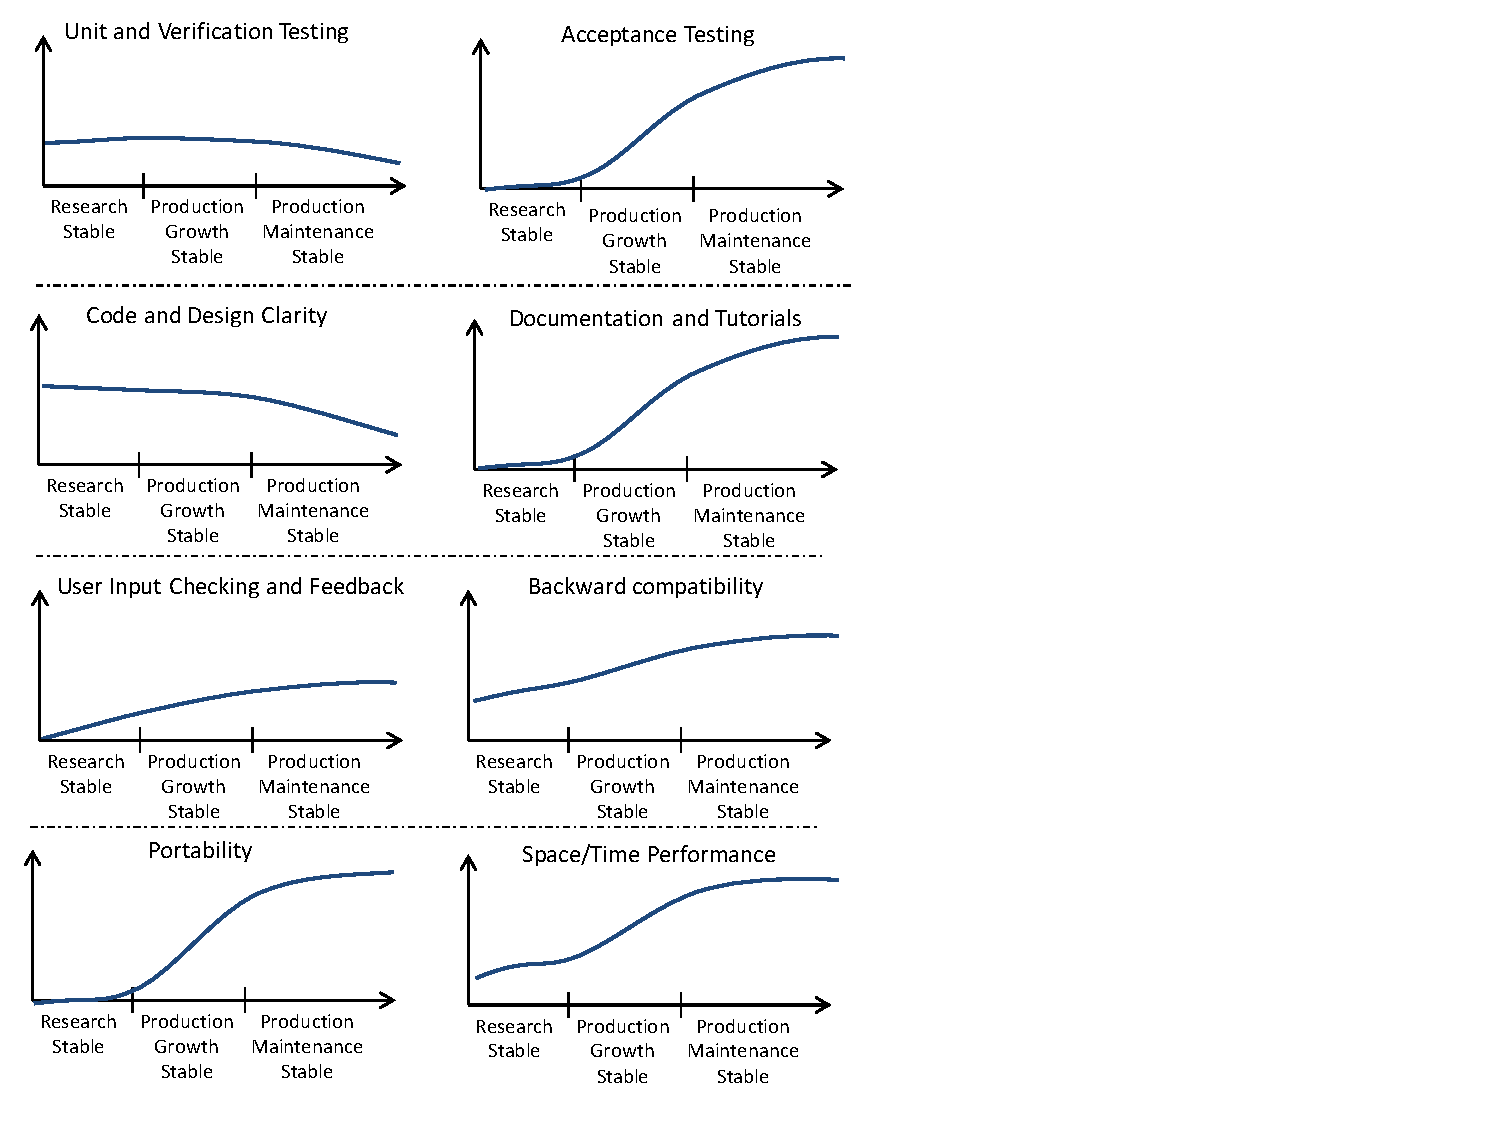
\includegraphics[trim = 0.1in 0.1in 4.0in 0.1in, scale=0.85]
{TypicalNonAgileSoftwarePhases}
%}
{}\caption{Example of the more typical variability in key quality
metrics in a typical CSE software development process.}
\label{fig:TypicalNonAgileSoftwarePhases}
\end{center}
\end{figure}

A typical non-Lean/Agile software development process used to develop
CSE software (as determined by personal experience and a number of
studies) would suggest that they have quality metrics like are shown
in Figure~\ref{fig:TypicalNonAgileSoftwarePhases} where unit and
verification testing and code/design clarity are low and only gets
worse with under maintenance.  The reduction in unit testing typically
occurs because as the software grows without maintaining a good
architecture, the entangling dependencies make it more and more
difficult to get objects into a test harness and the developers
invariably fall back on system level acceptance (or regression) tests.
At the same time, as the software is modified as new functionality is
added without being refactored, the software becomes more convoluted
and fragile and eventually dies the slow death of software
entropy~\cite{MythicalManMonth95}.

Note that the time-lines for user-oriented metrics for documentation,
acceptance testing, user input validation, backward compatibility,
portability, and performance would typically look more similar to a
Lean/Agile method as show in
Figure~\ref{fig:ImprovementsInDevelopmentPhases}.  The lack of typical
CSE projects to refactor their software might actually produce higher
levels of backward compatibility than the proposed Lean/Agile
lifecycle process being described here.  What is not shown in
Figure~\ref{fig:ImprovementsInDevelopmentPhases}, however, is the
added cost needed to get such a code to a higher quality state and
maintain it as more features are added.  Also, the lower the
design/code clarity and unit \& verification testing, the less likely
any group outside of the original development team can maintain the
software.

Depending on software such as this represents a large risk for
downstream customer projects since this software not self-sufficient
and is unsustainable any but the originating organization or team that
created the software.  The prevalence of this type of software in the
CSE community is a major reason for the trepidation that many CSE
groups have in taking on external software dependencies.  Most of this
apprehension is founded on real experiences of getting burned by bad
upstream CSE software.  The Trilinos lifecycle 2.0 model is an attempt
to reverse this tread (starting with Trilinos).


%
\section{Comparison to the Trilinos Lifecycle Model 1.0}
\label{sec:compare_with_lifecycle_1.0_model}
%

Here we discuss the similarities and differences to the originally
defined Trilinos lifecycle model {}\cite{TrilinosLifecycleModel2007}
which we will refer to here as Trilinos lifecycle 1.0 model, and the
new Trilinos lifecycle 2.0 model described in this document.

The Trilinos lifecycle 1.0 model defined three basic phases:

\begin{compactitem}

{}\item\textit{Research} Phase:

  \begin{compactitem}

  {}\item The research proposal is the project plan.

  {}\item Software is placed under configuration control as needed to
  prevent loss due to disaster.

  {}\item Peer reviewed published paper(s) is primary V \& V.

  {}\item The focus of testing is a proof of correctness, not
  software.

  {}\item Periodic status reports should be produced.

  {}\item A lab notebook, project notebook, or equivalent is the
  primary artifact.
  
  \end{compactitem}

{}\item\textit{Production Growth} Phase:

  \begin{compactitem}

  {}\item Agile methods (with associated lifecycles) are encouraged.

  {}\item All essential ASC SQE practices performed at an appropriate
  level (predetermined during promotion event from the research
  phase).

  {}\item Artifacts should naturally ``fall out'' from SQE practices
  and periodic status reviews and management reports.

  {}\item Process improvement and metrics are appropriate.
  
  \end{compactitem}

{}\item\textit{Production Maintenance} Phase:

  \begin{compactitem}

  {}\item Software has stable requirements.

  {}\item Most development is isolated to minor enhancements and bug
  fixes.

  {}\item Better design documentation and internal documentation are
  developed for the software.

  {}\item The software can be handed over to a different maintenance
  team.
  
  \end{compactitem}

\end{compactitem}

The Trilinos lifecycle 1.0 model also described specific promotional
events that require tasks such as risk analysis, gap analysis, and
explicit promotional decisions written up as semi-formal reports.
There is also mention of getting the team to seek more training
perhaps and the development of new processes.  The document
{}\cite{TrilinosLifecycleModel2007} mentions some set of required
practices and processes and supporting artifacts before a package has
been released (or get a waver from the Trilinos Project Leader).  It
is said that it is only after sufficient artifacts have been approved
that a package is eligible to go out in a Trilinos release.  Also, the
Trilinos lifecycle 1.0 model document says that once a package is no
longer supported that it will be removed from later Trilinos releases.

The biggest problem with the above described Trilinos lifecycle 1.0
model defined in {}\cite{TrilinosLifecycleModel2007} is that it is a
theoretical model.  The model is only theoretical because, as of this
writing, no Trilinos package has ever followed the outlined process of
performing documented risk analysis and gap analysis, and then
producing artifacts that are sent to the Trilinos framework list for
review and archiving.  No package has ever met the criteria necessary
for the Production Maintenance phase and no package has ever been
officially turned over to a ``maintenance support team.''  Packages
have only been abandoned by their primary developers without any plan
for future support and (for the most part) have still been allowed to
remain in subsequent Trilinos releases (with very few exceptions).
There are no modern SE lifecycle processes that advocate this type of
approach to developing software.  There is likely not even a single
Trilinos package that meets the criteria for the Production Growth
phase in {}\cite{TrilinosLifecycleModel2007} which includes the
specification for the use of Agile practices and the ``essential ASC
SQE practices'' (which are quite detailed) and there is no
documentation for what essential ASC SQE practices are followed and
which are not and why.

A primary substantive problem with the Trilinos lifecycle 1.0 model is
that it does not assume any quality software development practices are
being used while the software is first being developed in the Research
phase.  Mention of Agile (or any other) quality practices does not
come in until the Production Growth phase.  By that time, there may be
a significant amount of software that is well below standard in terms
of design/code clarity and unit and verification testing.  If this
software is used as the direct seed for the Production Growth phase
(which is what often happens), then there is typically such a large
technical debt that it never gets addressed once more focused efforts
towards productionization begin.  This is depicted in
Figure~\ref{fig:TypicalNonAgileSoftwarePhases} by the design/code
clarity and unit \& verification testing steadily going down as the
software is further developed.  The reason for this is discussed in
Section~\ref{sec:compare_with_typical_CSE_model}.  Software that
begins life with this level of (absent) standards is equivalent to the
Exploratory code category described in
Section~\ref{sec:life_cycle_overview} and
Section~\ref{sec:exploratory_code}.  As described in
Section~\ref{sec:research_stable_code}, it is possible for this type
of software to be refactored into a form that is appropriate for
production but that almost never happens in practice.  People and
funding agencies are not willing to pay down the technical debt and
there is just too much inertia with the current design and development
approaches and these plague the software for the rest of its existence
in challenged attempts to turn it into production software.  However,
if the software developed in the Research phase is completely
scrapped, it can be duplicated using Agile development practices as
described for Research Stable code in
Section~\ref{sec:research_stable_code}.  Therefore, the really only
hope for the Trilinos lifecycle 1.0 model is to completely scrap
software developed in the Research phase and rewrite it from scratch
in order to provide the seed for the Production Growth phase.

Another big difference between the 1.0 and 2.0 lifecycle models is
that the promotional event to the Production Maintenance phase.  In
the original 1.0 lifecycle model, the development team is supposed to
create a bunch of project artifacts after the fact and/or refactor (or
rewrite) much of the software from scratch.  This will likely never
happen, no-one will likely ever pay for this type of effort, and the
developers of the package will likely never do it.  Major batch
efforts left for the end of development are seldom ever actually done
in practice (hence ``small batch theory'' in Lean
{}\cite{ImplementingLeanSoftwareDevelopment}).  Instead, in this
updated lifecycle 2.0 model, preparing for maintenance mode is
accomplished incrementally by using Continuous Refactoring to keep
the design of the code simple and by creating and maintaining a
higher-level document that describes the key concepts as a road map
(examples of these types of high-level documents from the DDD book are
good).  Of course it is also facilitated by having very good unit and
other verification tests.  There is no need for the types of expensive
end-of-development artifacts that are described in
{}\cite{TrilinosLifecycleModel2007} if the software has the properties
of self-sustaining software (see
Section~\ref{sec:self_sustaining_open_source_software}).

Related to the issue of artifacts described above, yet another
difference between the original 1.0 and the current 2.0 Trilinos
lifecycle models is that in the 2.0 lifecycle model there are no
distinct promotional events or large batches of work necessary to move
a package from one lifecycle phase to the next like in the original
1.0 lifecycle model.  Instead, once enough of the attributes (e.g.,\
quality of documentation, error reporting, portability, etc.) of a
given lifecycle phase for a given package are met, a decision is made
by someone or some group of people that the package is in the next
stage and is then labeled as such.  The independent evidence inherit
in the software will support or refute such a claim and users can
assess such an assignment for themselves (more on this possible
assessment process in Section~\ref{sec:summary_next_steps} .

Another major problem with the Production Maintenance phase in the 1.0
lifecycle model is that there is an assumption that the software could
be redesigned and largely rewritten in order to allow the software to
endure long-term maintenance by a separate software support team.  The
problem with this assumption is the fact that you can't really
radically improve a piece of software with a redesign if you need to
maintain strong backward compatibility.  Inherit design flaws in the
user interface will never be fixable unless you deprecate problematic
aspects of the old user interface and replace them in a better design.

Another issue that is handled very differently between the Trilinos
1.0 and 2.0 lifecycle models is the issue equating ``release'' with
``production'' which was implicit in the original Trilinos lifecycle
1.0 model.  Instead, in the new 2.0 model, a Trilinos package can be
released (i.e.\ provided to a set of potential users that are not the
original developers) while being in any state of development.
However, making this work requires that Trilinos packages be properly
categorized so that users know what to (or not to) expect when taking
on a dependency on a Trilinos package.  For example, if it is
advertised that Trilinos package X is in the Exploratory phase,
potential customers know that they should not rely on or trust the
software in any way.  However, having access to such low-quality
research software can still be beneficial in order to help improve it
or use ideas from the software to create better quality software.  On
the other hand, if Trilinos package Y is categorized as Production
Maintenance code then users know that they can reply on the proper
functioning of the software and will also know that they will be able
to accept future versions of the software free of serious regressions
or changes in backward comparability.  In the new Trilinos lifecycle
2.0 model, releasing or not releasing software is not the issue.  The
issue is the proper categorization of the released software and
expressing the state of the software appropriately to prospective
users.  That puts the power in the hands of the user and they can make
up their own minds for how to deal with it different Trilinos
packages.

Another inconsistency between the Trilinos 1.0 and 2.0 lifecycle
models is that the 1.0 model's assertion that each Trilinos package
can have their own completely independent lifecycle model is
incompatible with the 2.0 lifecycle model's suggestion of providing an
official classification of Trilinos packages.  Without some official
uniform standards that come from these maturity level descriptions, end
users will be on their own trying to determine what Trilinos software
they should use and which they should wait until it becomes more
mature.

Finally, the last major difference between the 2.0 and 1.0 lifecycle
models is that the 2.0 lifecycle model does not assume that there is
any need for an official ``maintenance support team''.  The goal of
the 2.0 lifecycle model is the development of self-sustaining software
that can be maintained by anyone as needed and even by end users (who
then send patches back to the Trilinos support team).

However, the updated Lean/Agile lifecycle 2.0 model for Trilinos
described here does not totally invalidate the basic ideas in the
original Trilinos lifecycle 1.0 model but it does require a stronger
standard for fundamental testing and other basic Lean/Agile methods in
research software than what is currently in place in Trilinos (which
currently really has no standards for testing given that there are
released Trilinos packages with no automated tests at all and several
other packages have no tests in either an MPI or SERIAL build).


%
{}\section{Grandfathering of Existing Trilinos Code and Unspecified
Maturity}
\label{sec:grandfathering}
%

At the time of this writing, many of the established long-released
Trilinos packages don't meet the criteria for Stable code (not even
Research Stable not to mention Production Growth) because they lack a
sufficient level of unit and verification tests or the design and/or
internal structure of the software is too cluttered to be considered
self-sustaining software.  However, some of these established Trilinos
packages are hardened through extensive use by customers and bug fixes
and they are not as actively developed and therefore, for certain
common use-cases, are well verified.  This is a typical way in which
testing and hardening is performed in CSE and other domains but is not
consistent with Lean/Agile and does not lead to self-sustaining
software.  While all of this is true, we will have to ``forgive'' this
current generation of Trilinos packages and grandfather them into the
new lifecycle model.  At the same time, this code represents important
capabilities and needs to be maintained and improved.  Therefore, this
lifecycle model will allow these packages to be classified as Research
Stable, Production Growth, and Production Maintenance packages as long
as the package developers agree, from this point forward, to make all
further modifications to the code using high-quality Lean/Agile
consistent practicies.  The right way to maintain these important
packgaes going foward is to apply the Agile Legacy Software Change
algorithm defined in {}\cite{WorkingEffectivelyWithLegacyCode05} which
states that for every change to legacy code be carried out as follows:

\begin{compactenum}

{}\item\textit{Indentify Change Points}: Identify the code that needs
to change, issolate its change points and sensing points.

{}\item\textit{Break Dependencies}: Use hyper-sensitive minimal
editing to break fundamental dependencies to allow the code being
changed to be inserted into a unit test harness.

{}\item\textit{Cover with Unit Tests}: Write new unit tests to protect
the current functioning and behavor of the code that will be changed.

{}\item\textit{Add New Functionality with TDD}: Write new initially
failing unit tests to define the new desired behavior (or to reproduce
a suspected bug) and then change the code incrementally to get the new
unit tests to pass.  This is the test-driven development (TDD)
appraoch.  All the time, be rebuilding and rerunning the newly defined
unit tests to make sure changes don't break the existing behavior of
the code.

{}\item\textit{Refactor}: Clean up the code currently under test to
reduce complexity, improve comprehensibility, remove duplication, and
provide the foundation for further likely changes.

\end{compactenum}

The above algorithm can be shorted as ``cover'', ``change'', and
``refactor''.

Any existing package that will be further changed and maintained
according to the above-defined Agile Legacy Change algorithm can be
classified as follows:

\begin{compactenum}

{}\item Grandfathered Research Stable Code:

{}\item Grandfathered Production Growth Code:

{}\item Grandfathered Production Maintenance Code:

\end{compactenum}

By applying the above Agile Legacy Code change algorithm over and over
again in small chunks over a long period of time, even the worst
legacy software (i.e. with no tests and messy code) can slowly be
turned into quality software that will become easier to change.  If
grandfathered software is changed enough using the Agile Legacy Change
process, it may eventually achieve a level of design and clarity and
unit and verification testing that it can legitimately consider to be
Lean/Agile consistent software and the prefix ``Grandfathered'' can be
dropped.

On the other hand, if there are package development teams of existing
legacy software that are not committed to using the Agile Legacy
Change process to further maintain their code (and therefore
incrementally turn their software into self-sustaining software), then
their packages cannot be considered to be ``grandfathered'' into this
lifecycle model and therefore must be content to be categorized as
Unspecificed Maturity software.  In this case, the Trilinos project
will not comment in any official way at all on the quality or maturity
of a Trilinos package categorized as Unspecificed Maturity.  Trilinos
software classified as Unspecifided Maturity code requires that
prospective customers independently examine/test/evaluate the software
itself and/or directly communicate with the given package development
teams in order to determine quality in order to determine if they
should use the package or not.


%
{}\section{Summary and Next Steps}
\label{sec:summary_next_steps}
%

There needs to be a change in the way the CSE community writes
research-based CSE software including Trilinos software.  Much of the
current research software is of a state where there is not enough
confidence in the validity of the results to even justify drawing
conclusions in scholarly publications (there are some examples of
where defective software gave wrong results and hurt the creation of
knowledge in the research community
{}\cite{ScientistsNightmareFiveRetractions2006}).  CSE development
teams should be using TDD and need to write unit and verification
tests even if the only purpose of the software is to do research and
publish results.  There also needs to be some type of review of the
software to even provide the basis for publishing results that come
from the code (but of course the typical journal peer-review process
will not do this).

A follow-on to this document might be another document that defines an
official assessment process for Trilinos packages to assign their
current maturity level.  This assessment process would need to be
performed on a regular basis through code reviews and the examination
of various quality metrics.  Doing this would mean defining some
metrics that would then be applied in making these assessments. This
sounds much like a CMMI assessment but this is something that needs to
be considered.  One might just have a table of various metrics of
software quality and then maintain scores for the various Trilinos
packages.  Some of these metrics could be filled in automatically
(like code coverage) but most would be somewhat subjective and would
need people to make reasonable determinations.  The final
determination of a package's (or subpackages) phase / maturity level
could be determined by the minimum score in a given category or by
some other criteria.

Assuming Trilinos could officially assign maturity levels based on
well defined quality metrics, in order to be useful, Trilinos packages
would have to be explicitly tagged by their currently assessed
lifecycle maturity level, e.g., Exploratory, Research Stable,
Production Growth, or Production Maintenance.  This would be
facilitated by officially tagging Trilinos packages in the CMake build
system so that someone, for example, could enable all Production
Maintenance code with
{}\ttt{Trilinos\_ENABLE\_MINIMUM\_MATURITY\_LEVEL =
PRODUCTION\_MAINTENANCE} and all software that does not achieve that
level of maturity would be disabled.  Actually, in order to allow new
capabilities to be constantly developed in existing Trilinos packages,
the lifecycle phase should be assigned to subpackages within a
Trilinos package to allow software of lower maturity to coexist in the
same package with more mature software.  For example, a package
labeled as Production Maintenance could have one subpackage at the
level Production Maintenance but could also have another subpackage at
the level Production Growth and another at Research Stable or even
Exploratory maturity level.  Therefore, when Trilinos is configured
with {}\ttt{Trilinos\_ENABLE\_MINIMUM\_MATURITY\_LEVEL =
PRODUCTION\_MAINTENANCE}, only the one Production Maintenance
subpackage would be enabled.  However, when Trilinos was configured
with {}\ttt{Trilinos\_ENABLE\_MINIMUM\_MATURITY\_LEVEL =
RESEARCH\_STABLE}, then the Production Maintenance, Production Growth,
and the Research Stable subpackages would all be enabled.  In this
way, users could explicitly filter Trilinos software according to the
required level of maturity before deciding what Trilinos packages to
depend on and which are not yet ready for their usage.  The utility of
such a configure time option should be determined by polling Trilinos
customers.  Supporting such a feature would require adding just three
new nightly builds for the different values of
{}\ttt{Trilinos\_ENABLE\_MINIMUM\_MATURITY\_LEVEL} of
{}\ttt{RESEARCH\_STABLE}, {}\ttt{PRODUCTION\_GROWTH}, and
{}\ttt{PRODUCTION\_MAINTENANCE} would these extra tests would only be
needed on a single platform so would not significantly increase
testing overhead.

Finally, as mentioned in Section~\ref{sec:grandfathering}, existing
Trilinos packages will necessarily need to be ``grandfathered in''.
This newly defined lifecycle process will not magically get everyone
who develops Trilinos software to develop their software in a
Lean/Agile consistent way (i.e.\ with high unit and verification
testing right from the very beginning with a clean code base).  There
is a large cultural issue that will need to be addressed and this
document is just a step along the path to get the CSE community (and
the Trilinos development community in particular) to where it needs to
be with respect to software quality in Trilinos and related CSE
software.


% ---------------------------------------------------------------------- %
% References
%
\clearpage
\bibliographystyle{plain}
\bibliography{references}
\addcontentsline{toc}{section}{References}

% ---------------------------------------------------------------------- %
% Appendices should be stand-alone for SAND reports. If there is only
% one appendix, put \setcounter{secnumdepth}{0} after \appendix
%
%\appendix

%
% Glossary
%

%\section{Glossary}

%Blah, blah, blah ..

%
% Index
%

%\addtocontents{toc}{~  ~ ~  ~ Index}
%\printindex

%\begin{SANDdistribution}
%\end{SANDdistribution}

\end{document}
